\section{Access Controll}
\subsection{Multi Protocol Access (Synapse)}
\gls{ADL} ist kompatible mit \textit{Hadoop}. Die Daten können verwaltete und auf sie zugegriffen werden, wie im bei einem \gls{HDFS}. Der Driver \gls{ABFS} ist in allen \textit{Apacha Hadoop} Umgebungen verfügbar, so auch bei \textit{Azure Bricks und HDInsight}. Der Driver \gls{ABFS} ist auf Daten Analyse optimiert.\\

Eine andere Möglichkeit auf die Daten zuzugreifen ist, ist über ein klassischen Blob Storage \gls{API} Zugang mit \gls{WASB}. Services wie Power BI erlauben beide Protokolle.

\begin{figure}[H]
	\centering
	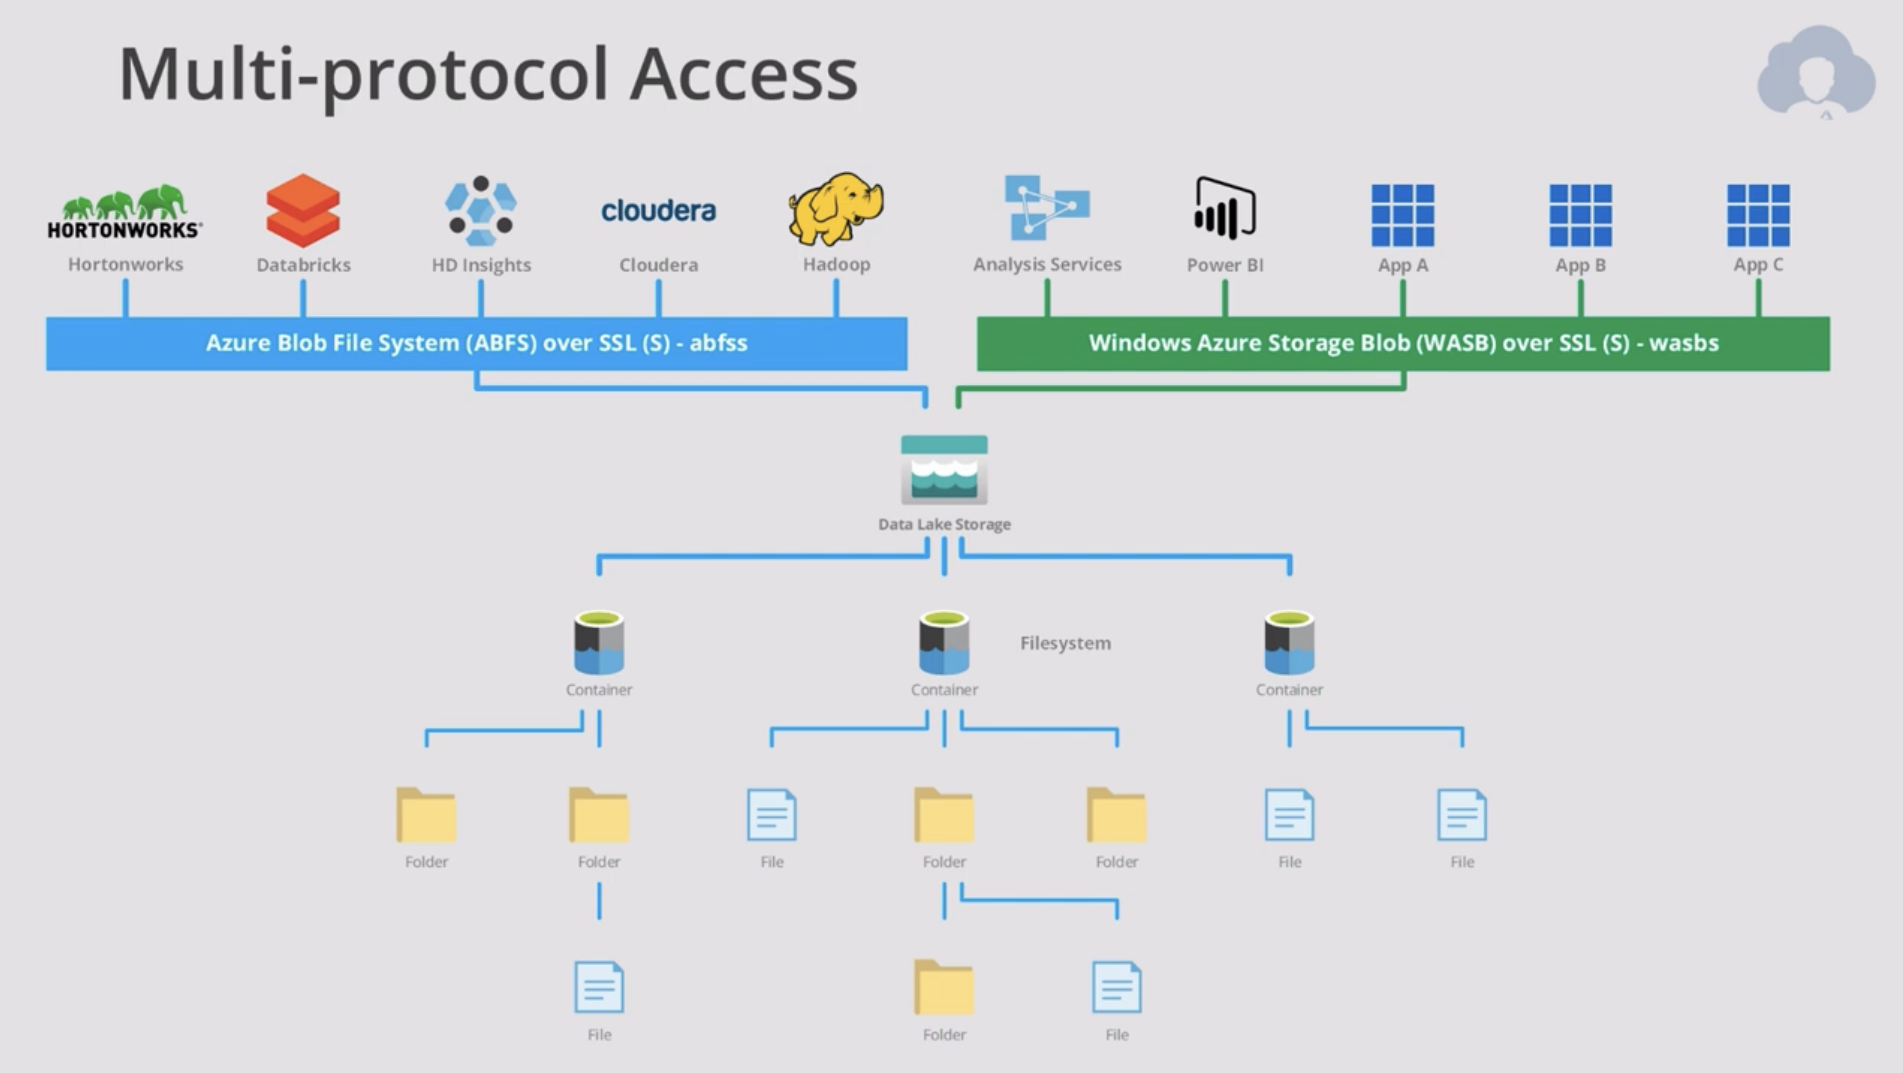
\includegraphics[scale = 0.4]{attachment/chapter_2/Scc111}
\end{figure}


\subsection{Data Access though Storage Explorer}
Im Browser kann über \textit{Storage Explorer}
\begin{figure}[H]
	\centering
	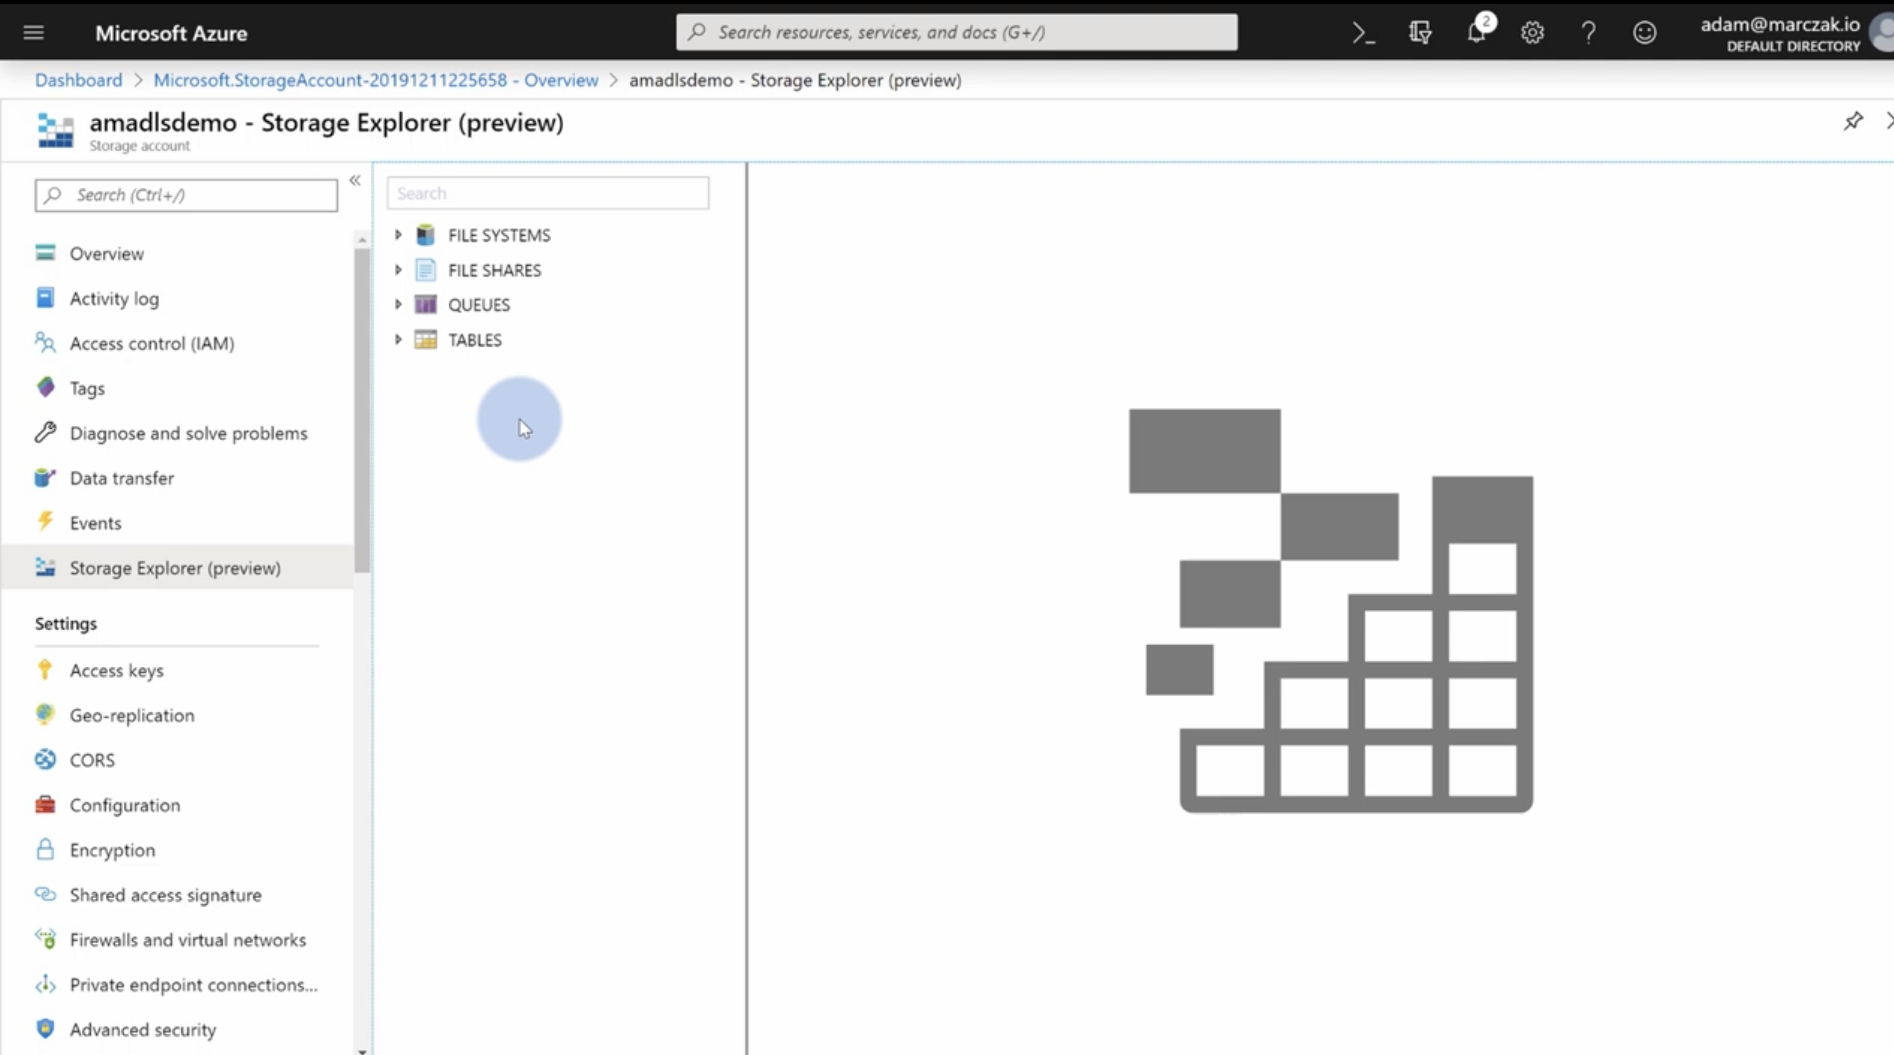
\includegraphics[scale = 0.2]{attachment/chapter_2/Scc116}
\end{figure}

oder direkt über \textit{Storage Explorer}

\begin{figure}[H]
	\centering
	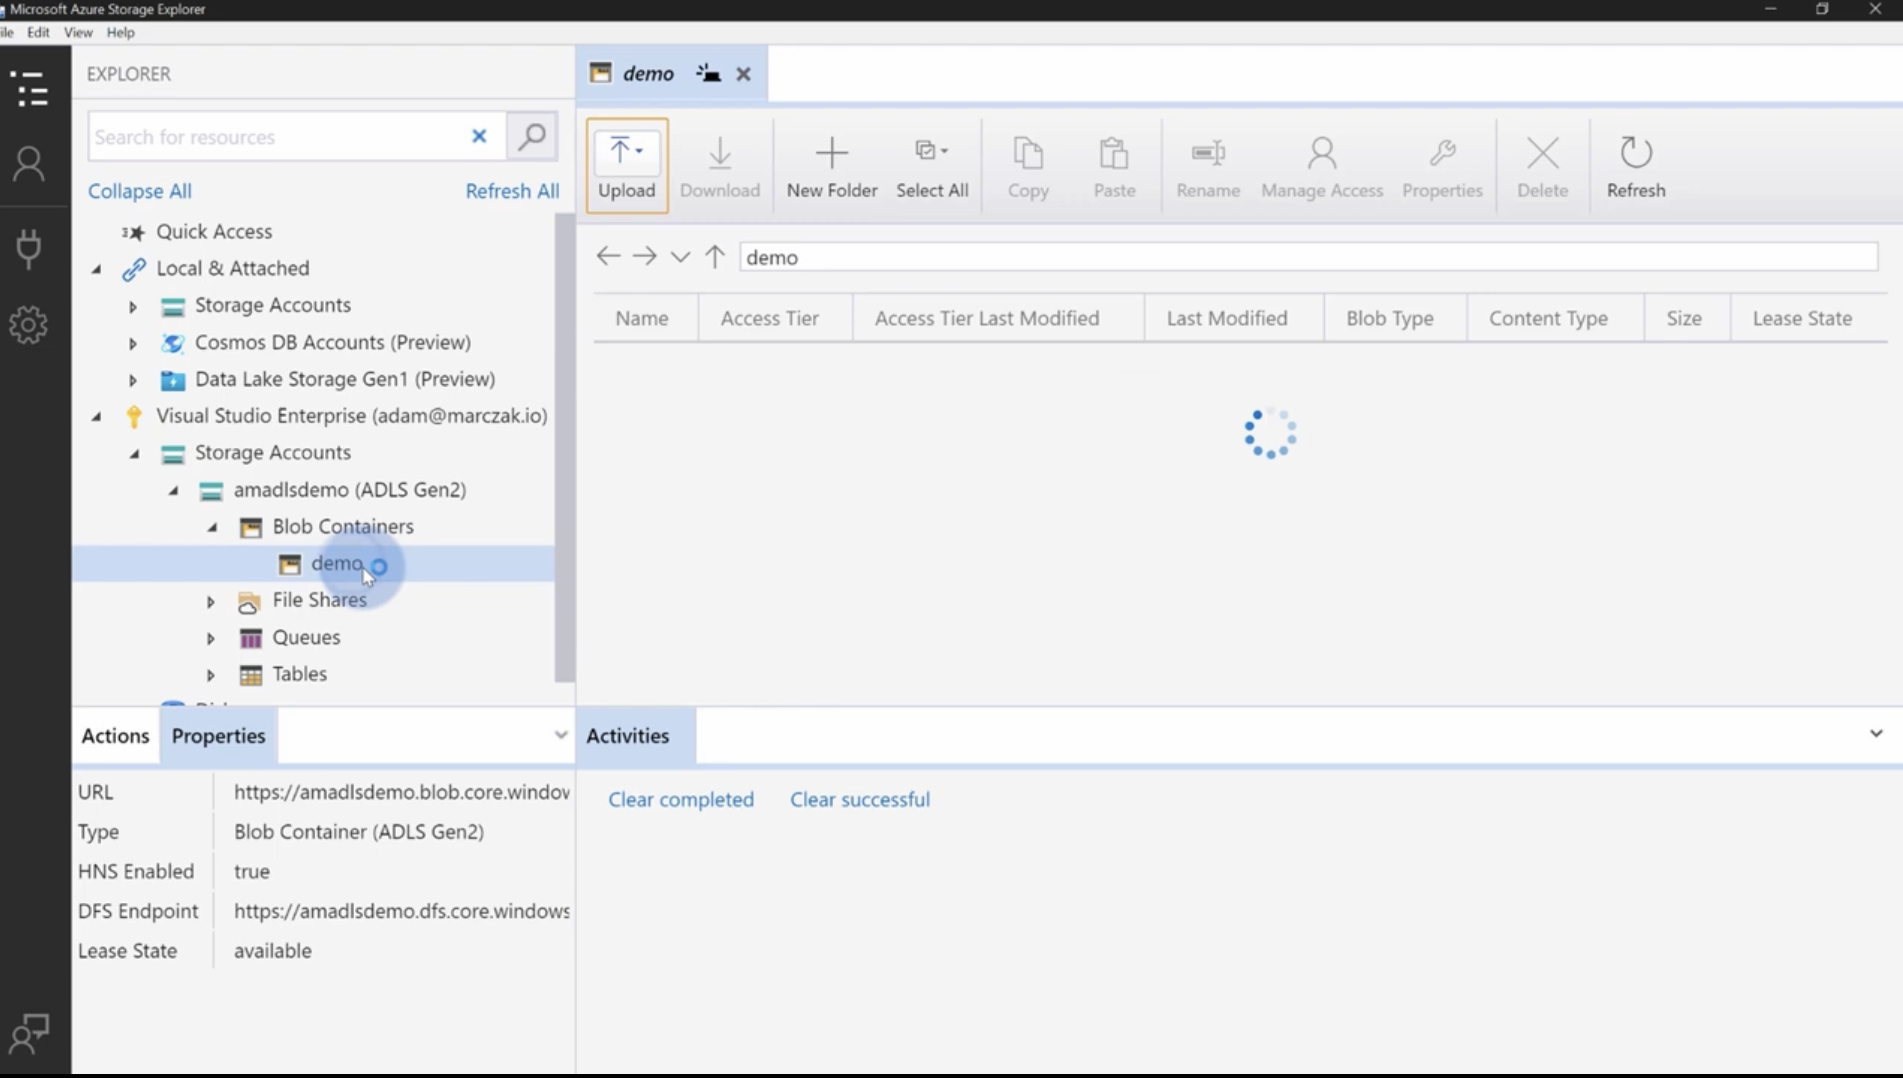
\includegraphics[scale = 0.2]{attachment/chapter_2/Scc117}
\end{figure}
eingesehen werden.\\

\subsection{Access control lists (ACLs)}
Das Zugriffsmodell für \gls{ADL} erlaubt
\begin{itemize}
	\item \gls{RBAC} und
	\item \gls{ACL}.
\end{itemize}

Im Fall von \gls{ACL} besitzt jede Datei und Verzeichnis eine Liste, welche den Zugriffsberechtigungen enthält. Dieser kann über mehrere Quellen hinterlegt werden.

\begin{figure}[H]
	\centering
	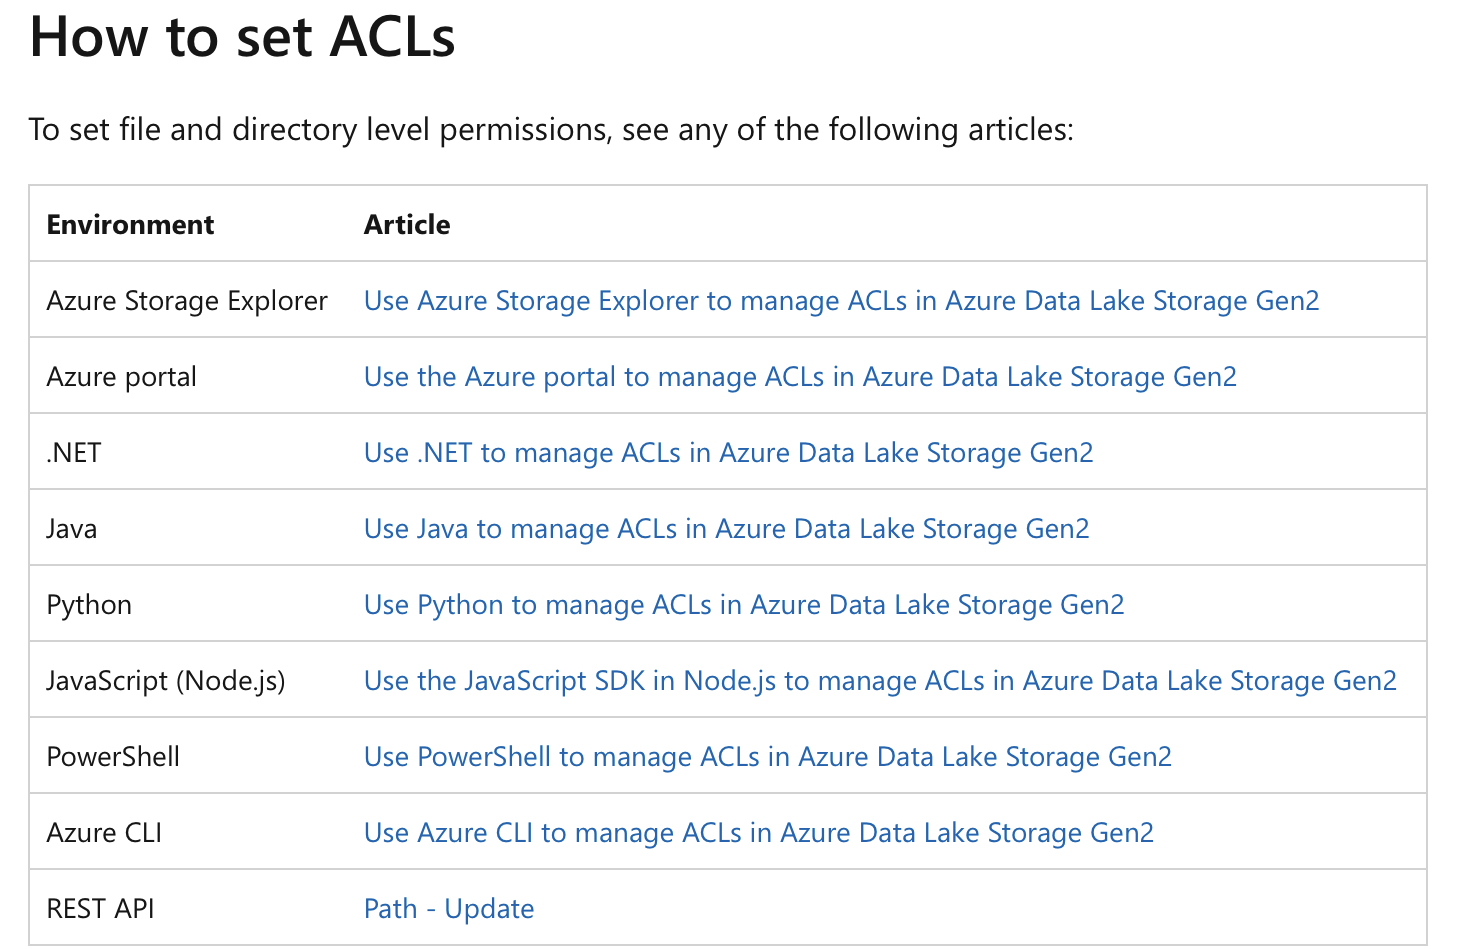
\includegraphics[scale = 0.2]{attachment/chapter_2/Scc119}
\end{figure}

Am Beispiel des \textit{Azure Storage Explorer} sieht dies wie folgt aus: Der Zugriff (\textit{Manage Access}) für Dateien oder Ordner kann für User mit verschiedenen Berechtigungen gemanaget werden.
	\href{https://learn.microsoft.com/en-us/azure/storage/blobs/data-lake-storage-access-control-model#access-control-lists-acls}{Quelle}

\begin{figure}[H]
	\centering
	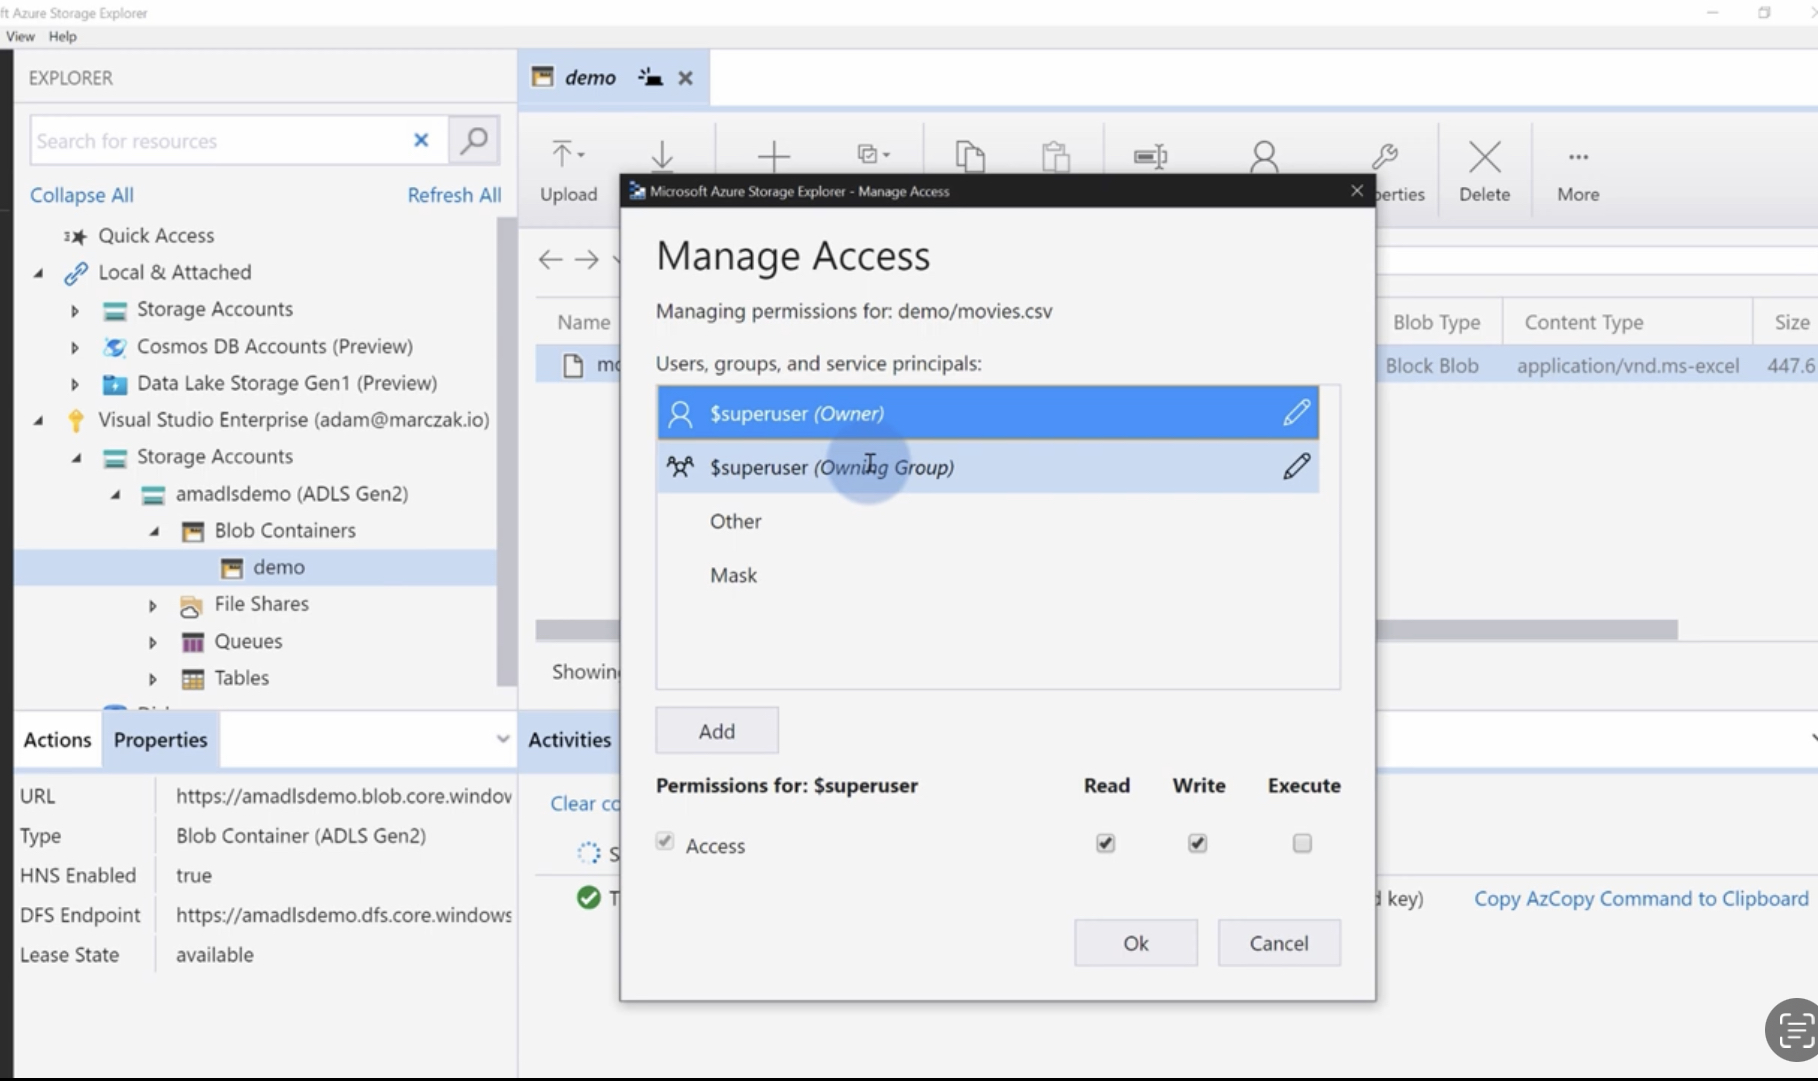
\includegraphics[scale = 0.2]{attachment/chapter_2/Scc118}
\end{figure}

\subsection{Role Based Access Control (RBAC}
Kernbegriffe
\begin{itemize}
	\item Role (Definition),
	\item Role Assignment,
	\item Security Principal,
	\item Scope
\end{itemize}

Mit und über die verfügbaren Ressourcen in Azure können Aktionen (Actions) ausgeführt werden. Um die Vielfalt der möglichen Aktionen zu bündeln, gibt es das Konzept einer Role.
\footnote{
	\href{https://youtu.be/4v7ffXxOnwU}{Quelle}
}

\begin{center}
	Definition: Role - A Role is a collection of action, that a assigned identity can be performing.	
\end{center}

Die Aktionen werden auf Azure in vorkonfigurierten Rollen festgehalten. Neue Rollen können aber angelegt werden.
\begin{figure}[H]
	\centering
	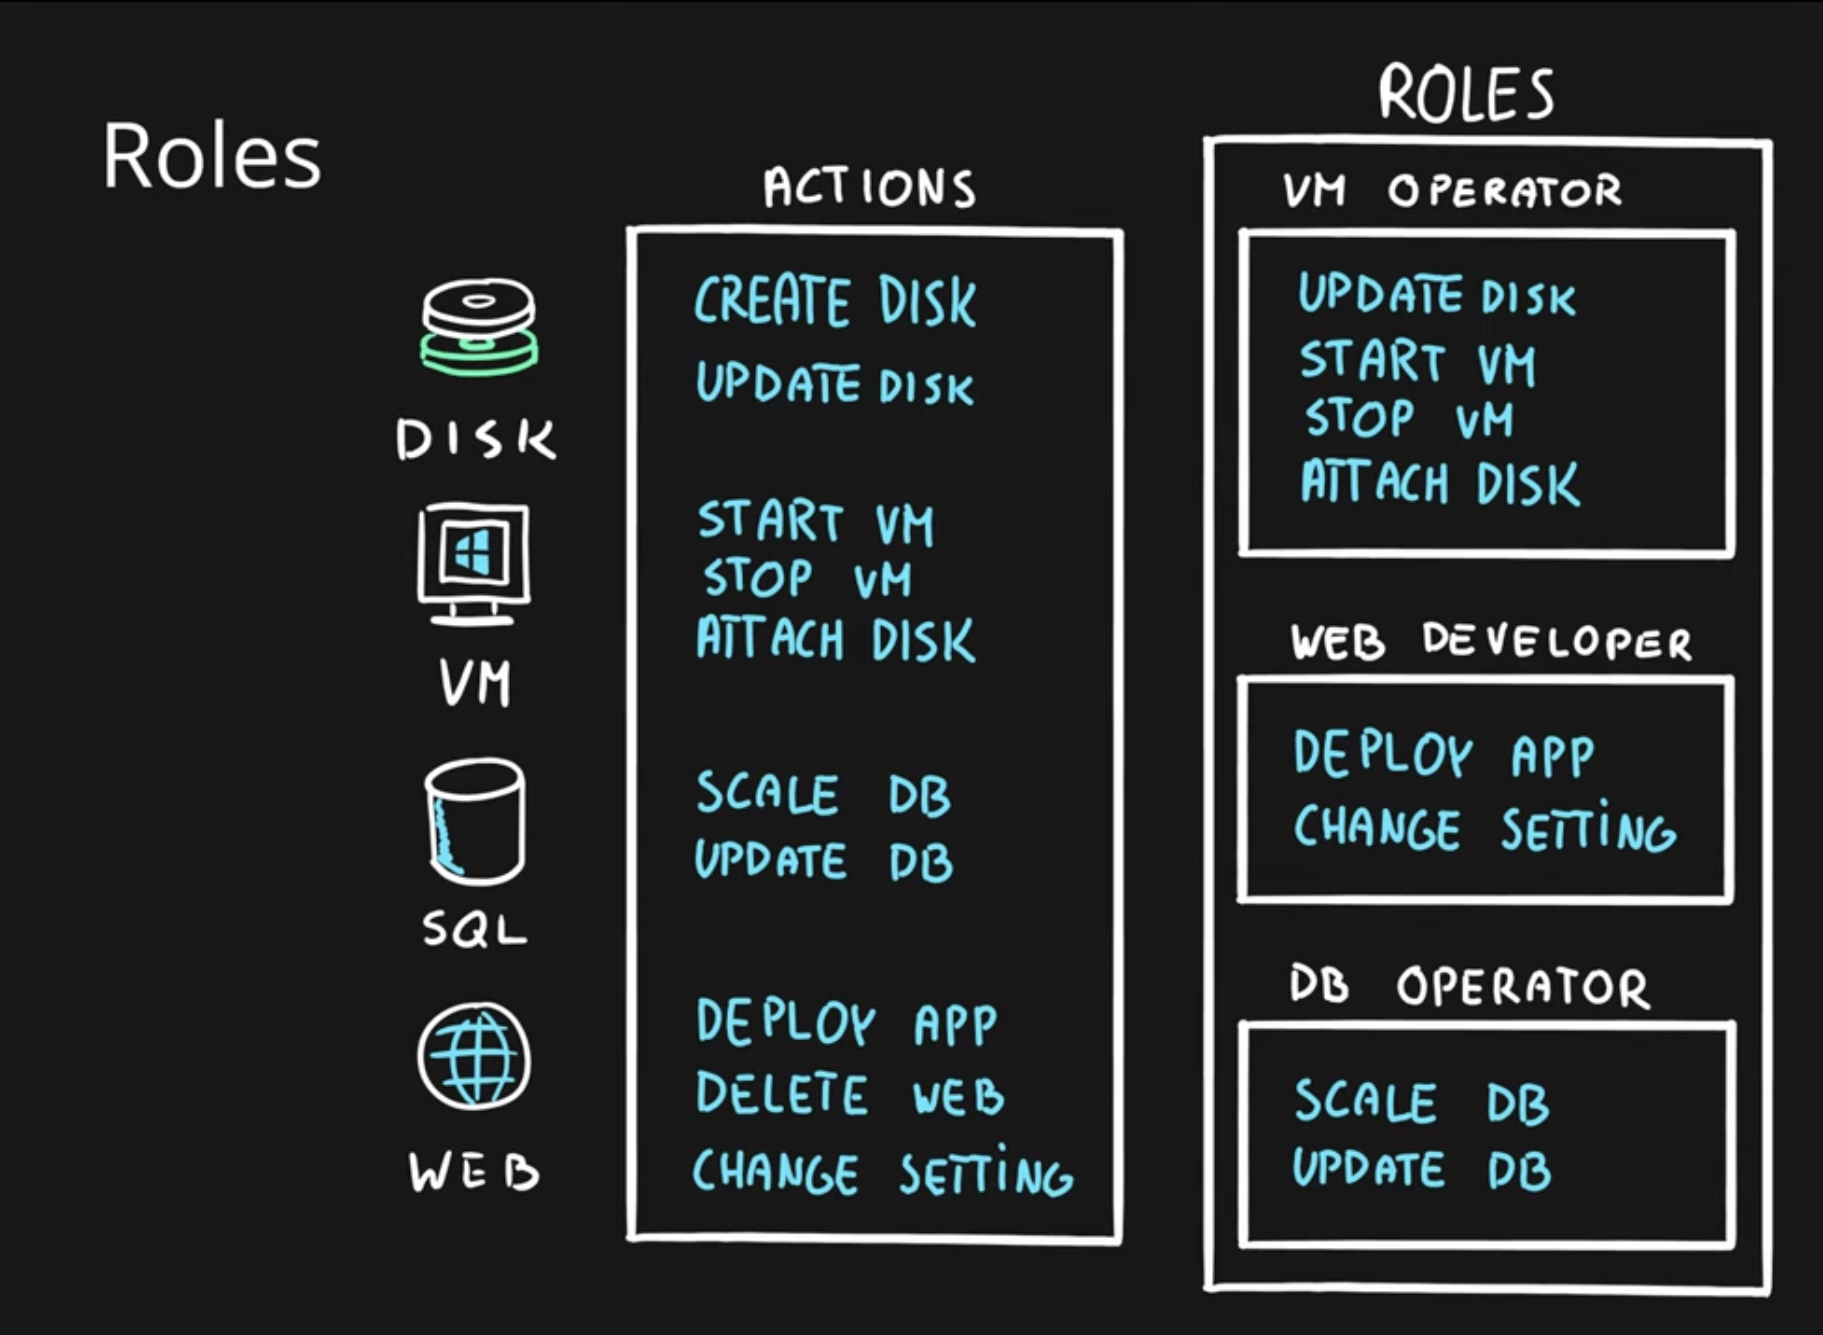
\includegraphics[scale = 0.2]{attachment/chapter_2/Scc120}
\end{figure}

\begin{figure}[H]
	\centering
	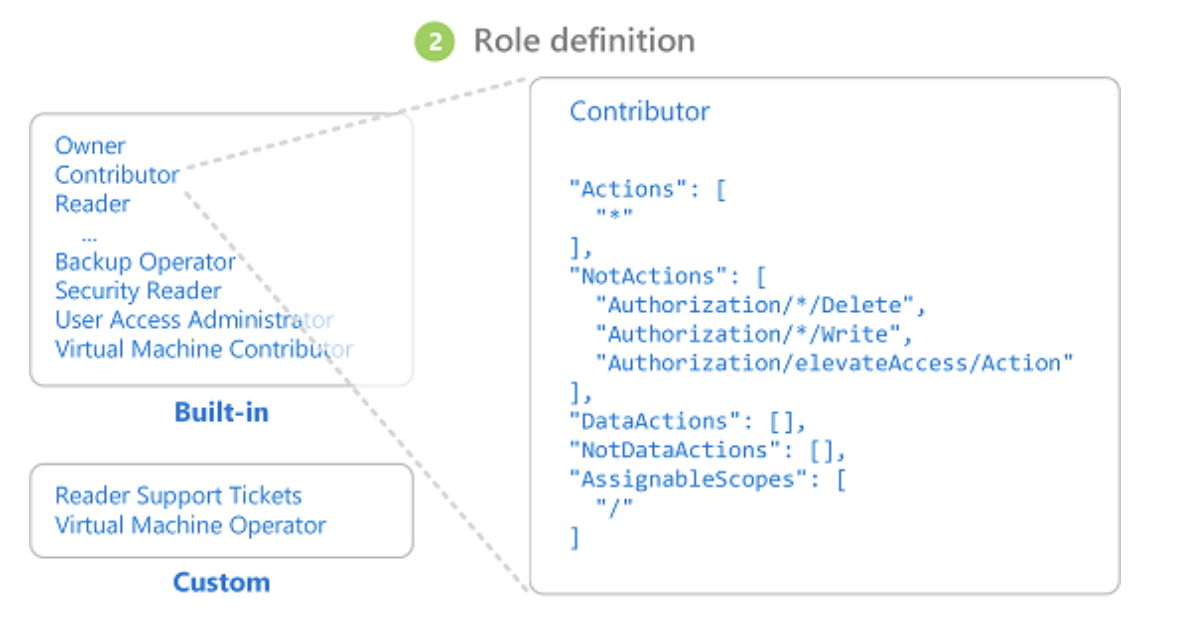
\includegraphics[scale = 0.2]{attachment/chapter_2/Scc123}
\end{figure}

Eine Role kann einem \textit{Security Principal} zugewiesen werden. Ein \textit{Security Principal} ist eine Objekt welches ein
\begin{itemize}
	\item User,
	\item User Group,
	\item Service Principal oder 
	\item Manage Identiy
\end{itemize}
sein kann.

\begin{figure}[H]
	\centering
	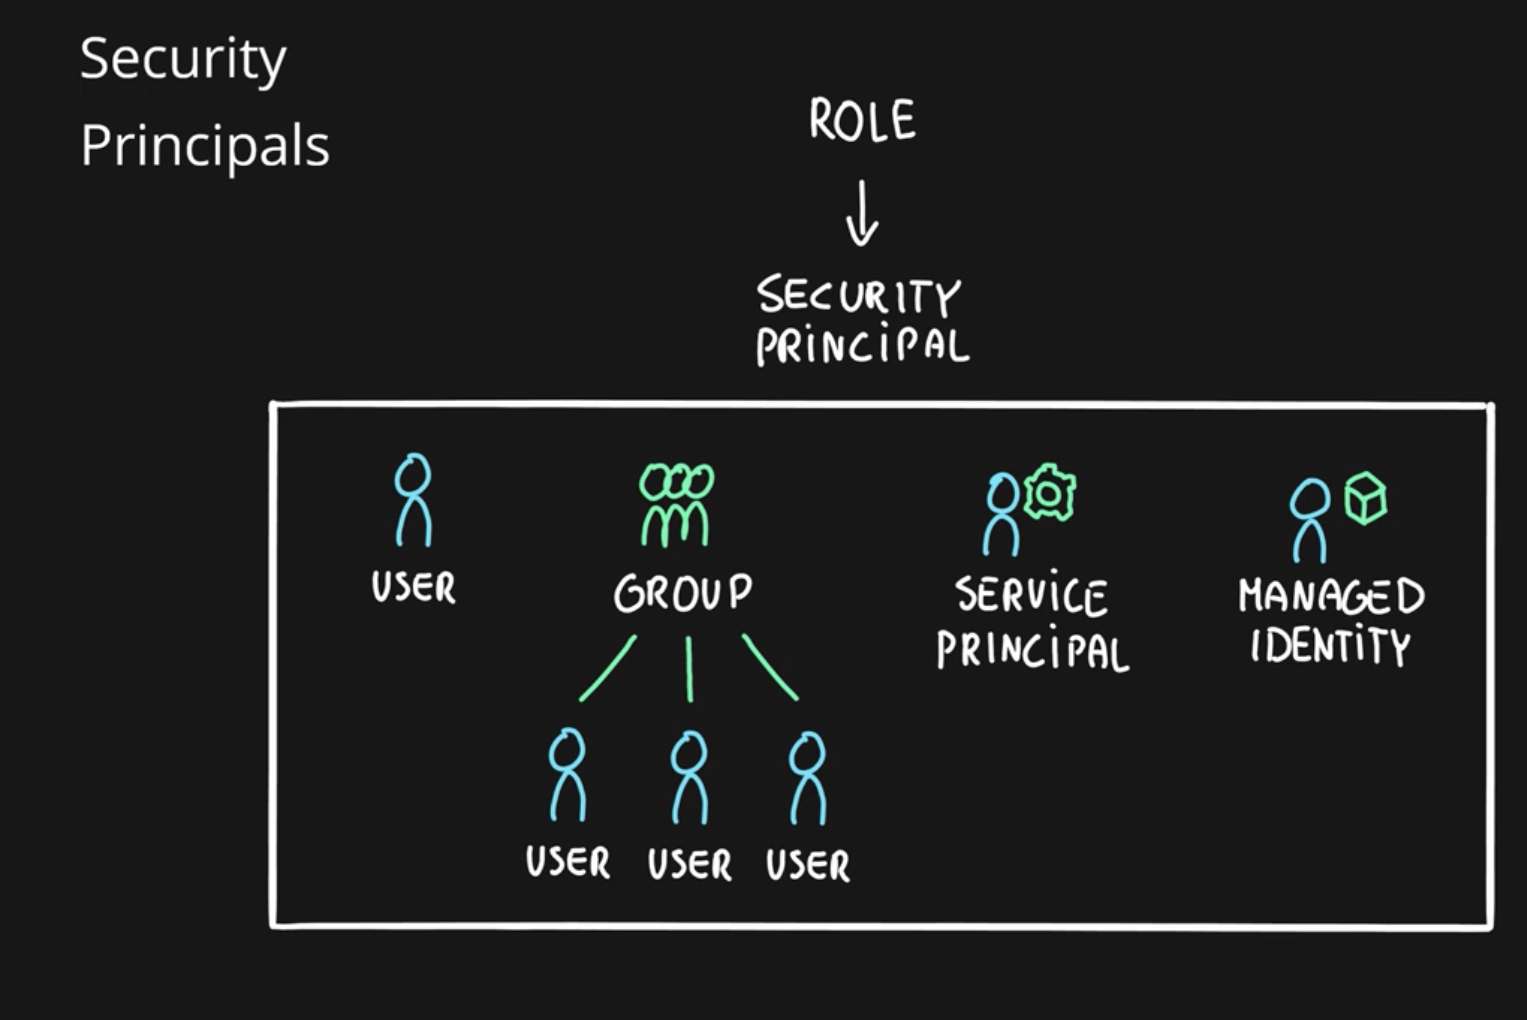
\includegraphics[scale = 0.2]{attachment/chapter_2/Scc121}
\end{figure}

Dieses Objekt erhält
\begin{itemize}
	\item Berechtigungen auf eine eine Ressource und 
	\item und kann eine \textit{Rolle} zugewiessen bekommen. 
\end{itemize} 

\begin{figure}[H]
	\centering
	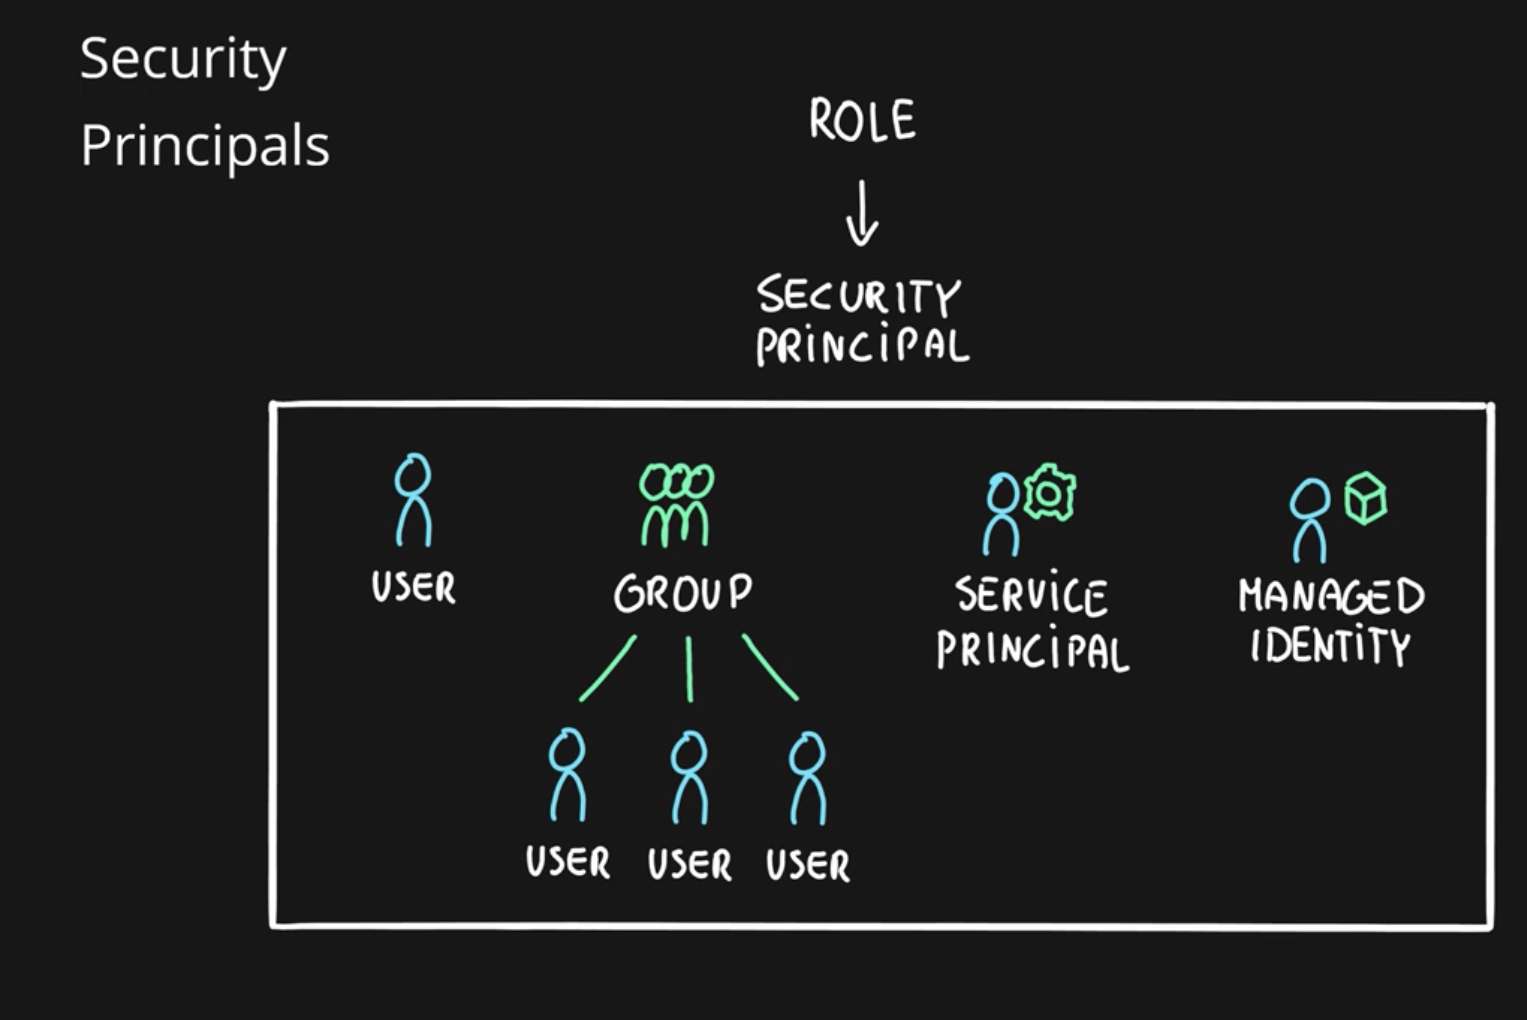
\includegraphics[scale = 0.2]{attachment/chapter_2/Scc121}
\end{figure}

Um das Thema \textbf{Scope} zu verstehen, ist die Struktur von Azure zu verstehen.
Der Aufbau von \textit{Azure} gestaltet sich wie folgt
\begin{center} 
	\item Manage Group > Subscription > Resource Group > Ressource
\end{center}

\begin{figure}[H]
	\centering
	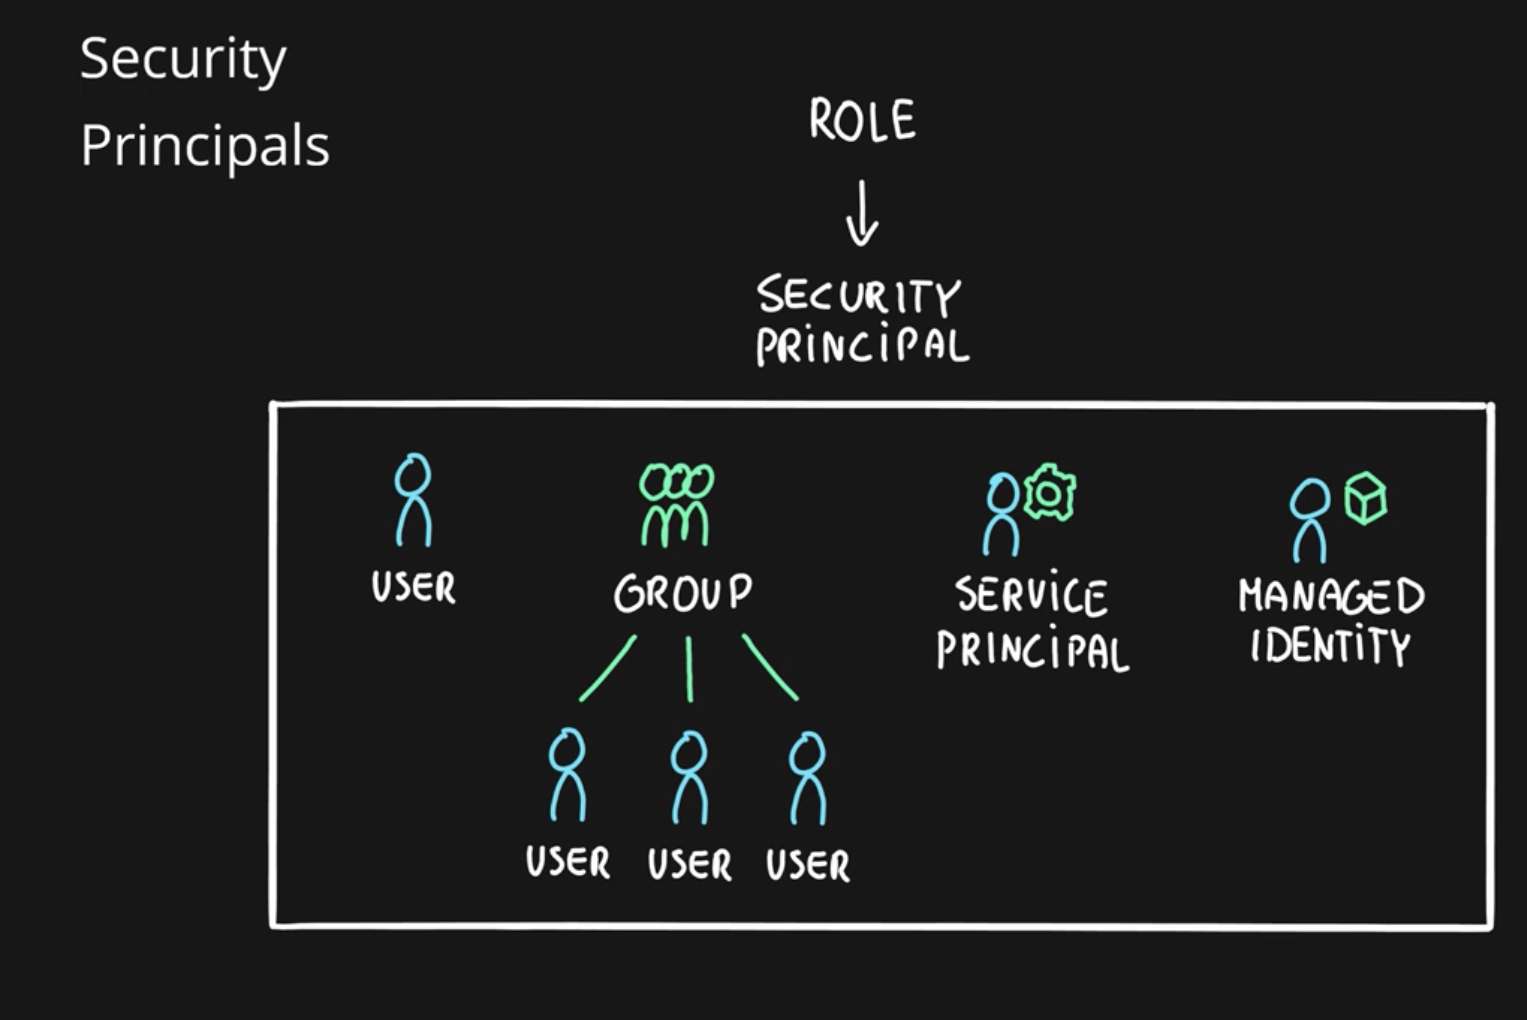
\includegraphics[scale = 0.2]{attachment/chapter_2/Scc121}
\end{figure}

Unter einer \textit{Subscription} hat den Zweck die Menge und den Kostenverbrauch für die angebundenen Ressourcen zu managen.\\

Eine \textit{Resouce Group} hat den Zweck, alle Ressourcen zu bündeln, welche den gleichen Lebenszyklus besitzen. Dies soll es leichter machen Deployments, Löschungen und Update gleichzeitig für alle unterliegenden Ressourcen durchzuführen.\\

Wie schon erwähnt, kann eine Rolle einem \textit{Security Principal} zugewiesen werden. Eine Role kann auch einem \textit{Scope} zugewiesen werden. Bei einer Zuweisung gilt das Prinzip der \textit{Vererbung}.
\begin{figure}[H]
	\centering
	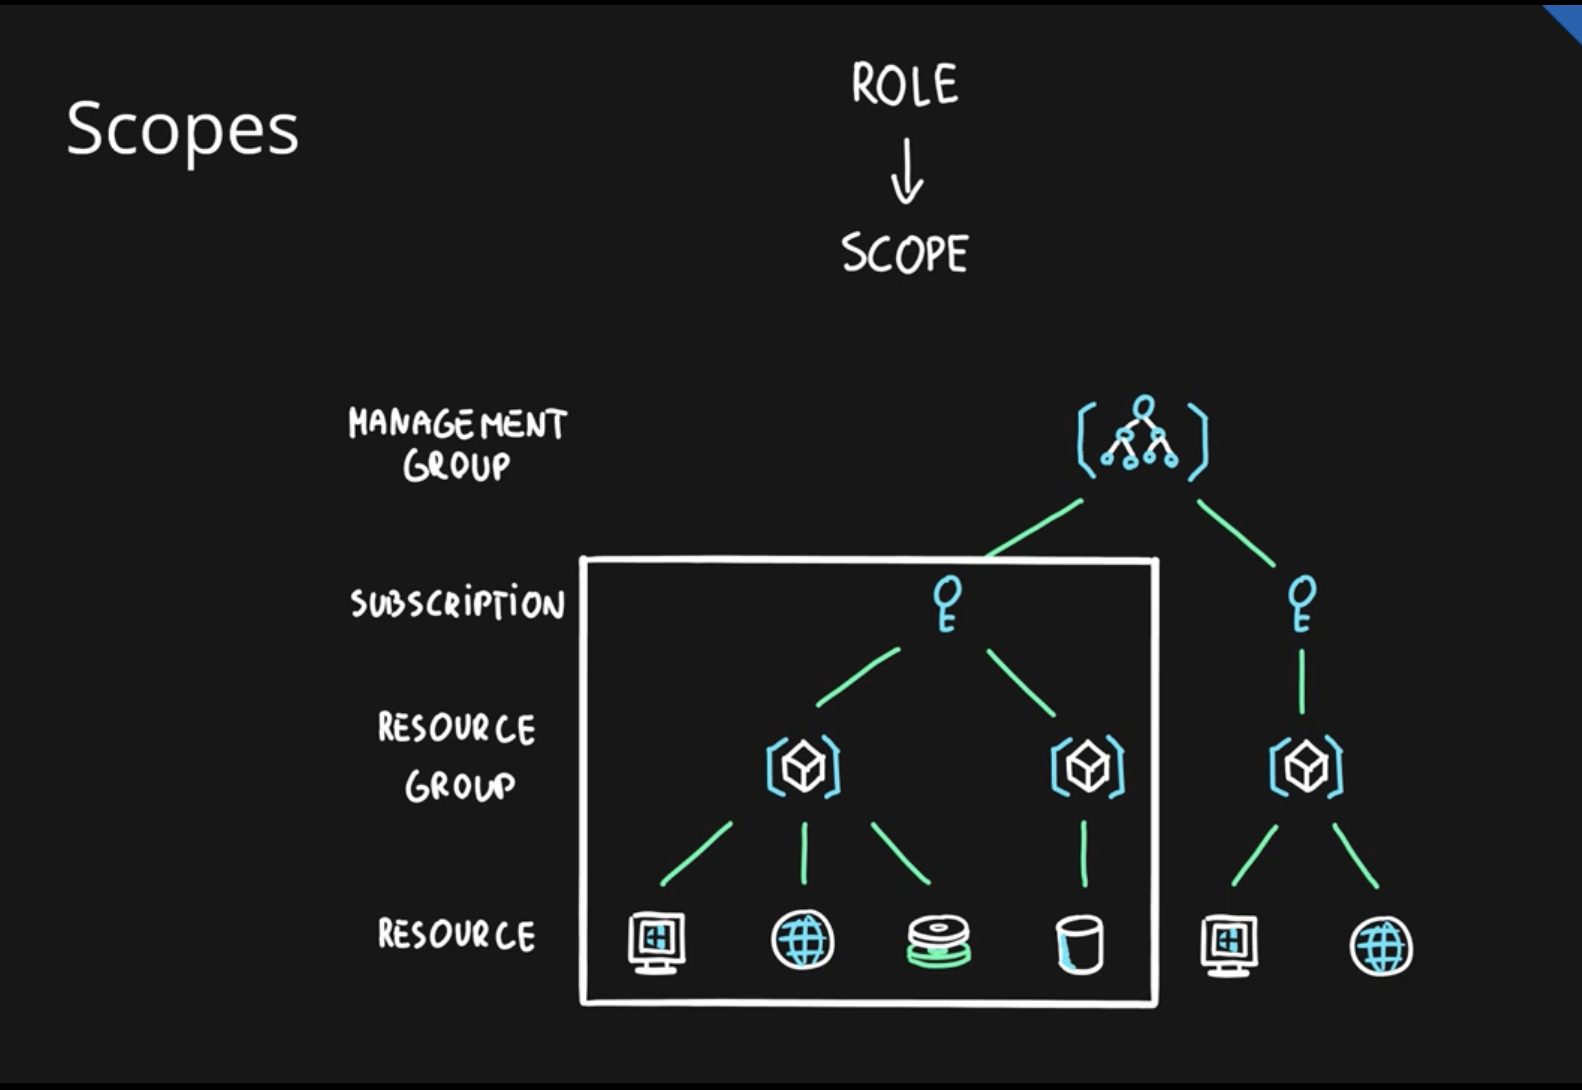
\includegraphics[scale = 0.2]{attachment/chapter_2/Scc124}
\end{figure}

Ein hierachiesch höhere Ressource vererbt der ihr untergeordneten Ressourcen die Rollen Zuweisung.\\

Die Kombination aus 
\begin{itemize}
	\item Aktionen bündeln (Role),
	\item Zuweisung einer Role eines \textit{Security Principal} und
	\item Zuweisung einer Role eines \textit{Scope}
\end{itemize}
wird als \textbf{Role Assignment} bezeichnet.

\subsection{Example Power BI Multi Protocol Access}
Mit \gls{ADL} kann mit den \textit{Multi Process Access} über mehrere Connectoren verbunden werden.

\begin{figure}[H]
	\centering
	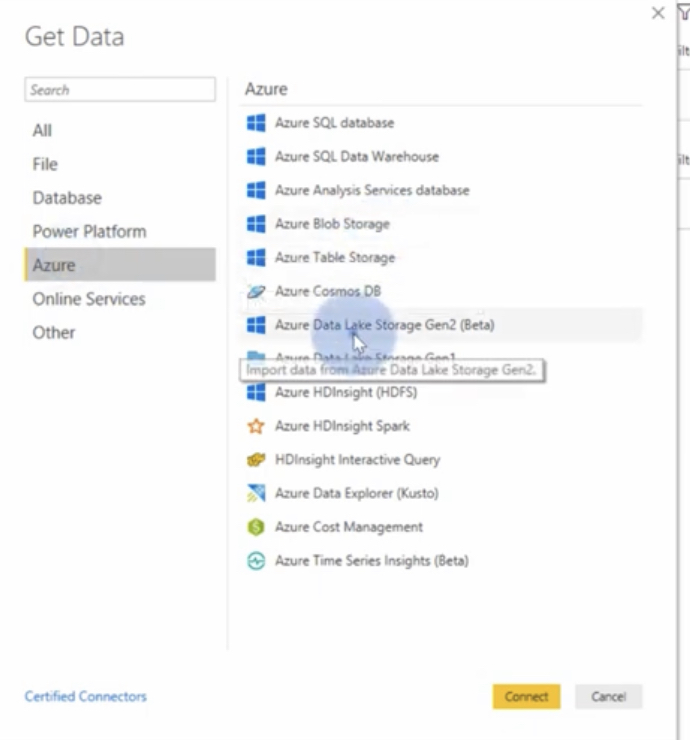
\includegraphics[scale = 0.2]{attachment/chapter_2/Scc125}
\end{figure}

Die Informationen für den Endpunkt von \gls{ADL} kann unter \textit{Azure Portal/Ressources/Azure Data Lake/Properties} nachgeschaut werden.

\begin{figure}[H]
	\centering
	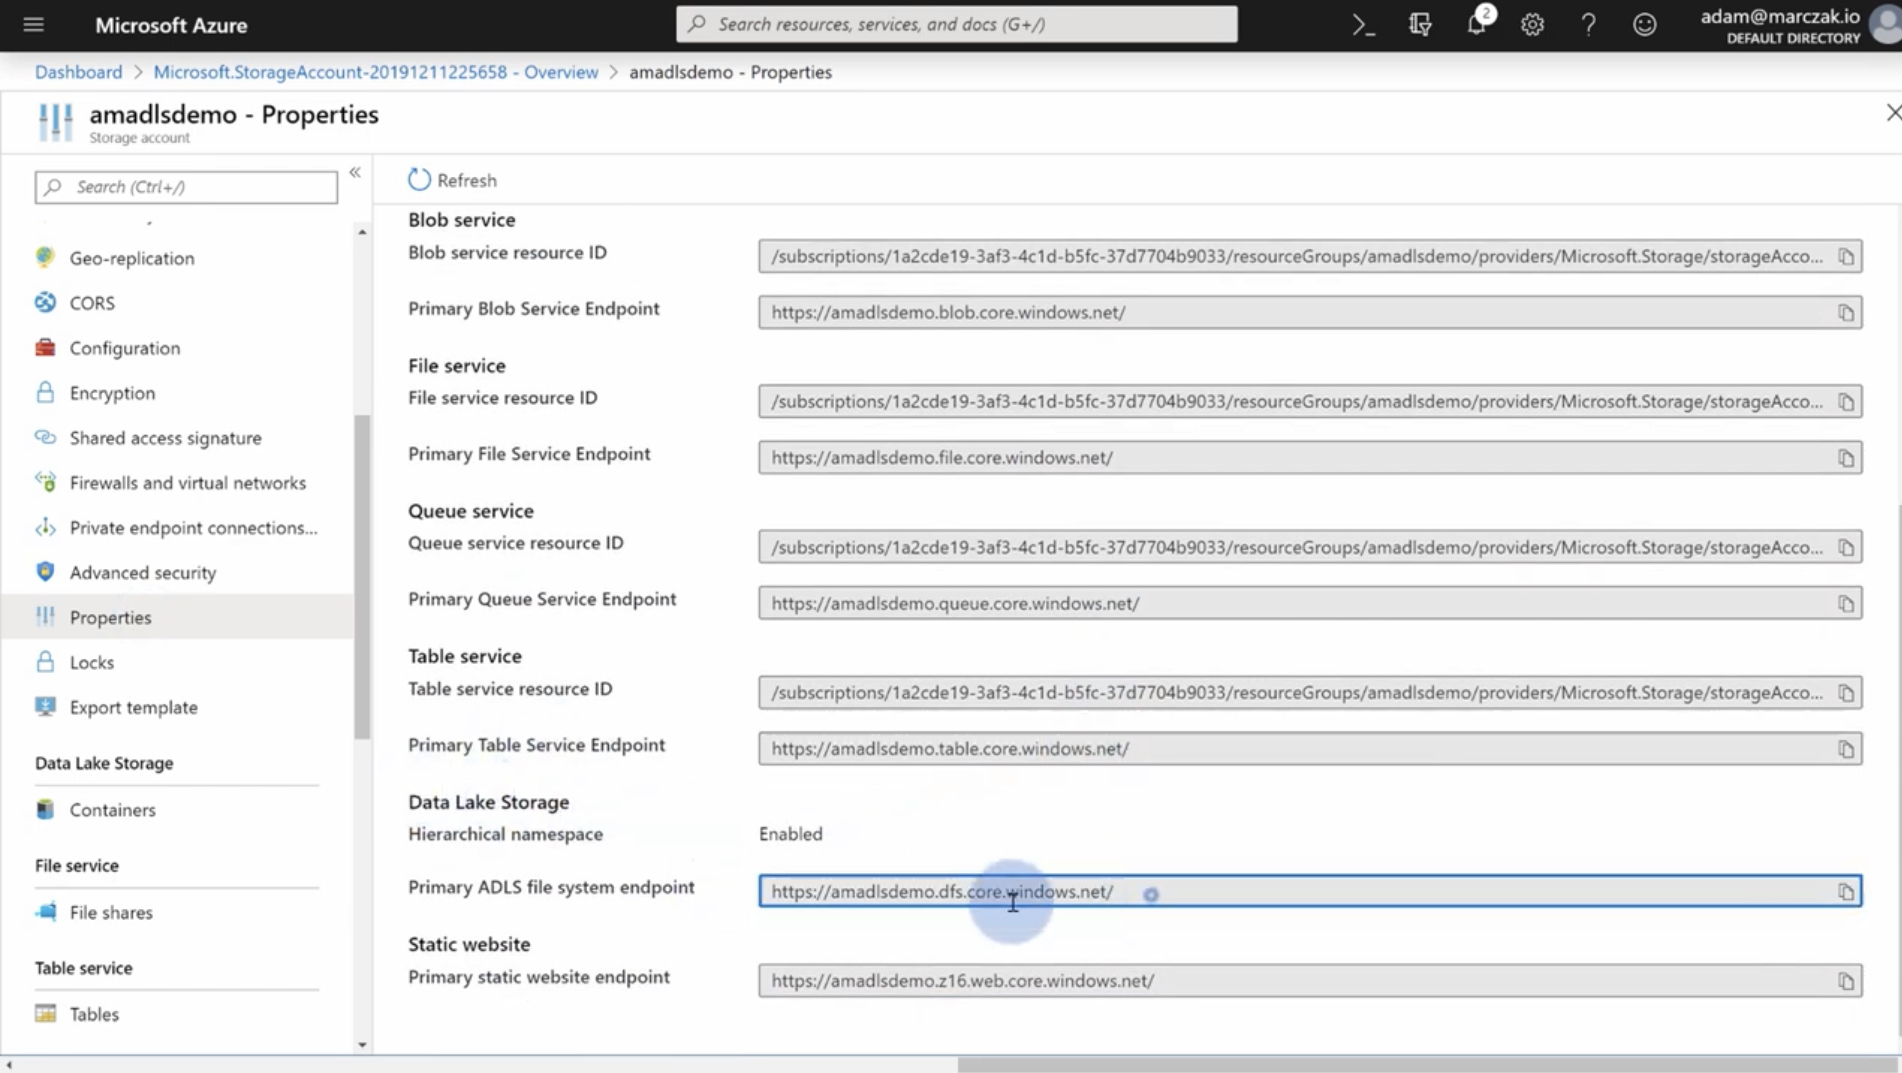
\includegraphics[scale = 0.2]{attachment/chapter_2/Scc126}
\end{figure}

Es kann sich über den User angemeldet werden. Ebenso kann ein \textit{Konto-Schlüssel (Account key)} verwendet werden.

\begin{figure}[H]
	\centering
	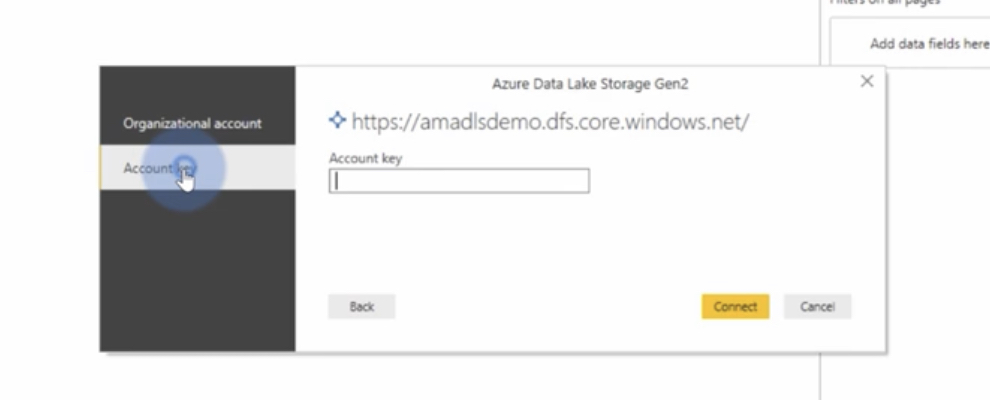
\includegraphics[scale = 0.2]{attachment/chapter_2/Scc128}
\end{figure}

Dieser kann über \textit{Azure Portal/Ressources/Azure Data Lake/Access Keys} eingesehen werden

\begin{figure}[H]
	\centering
	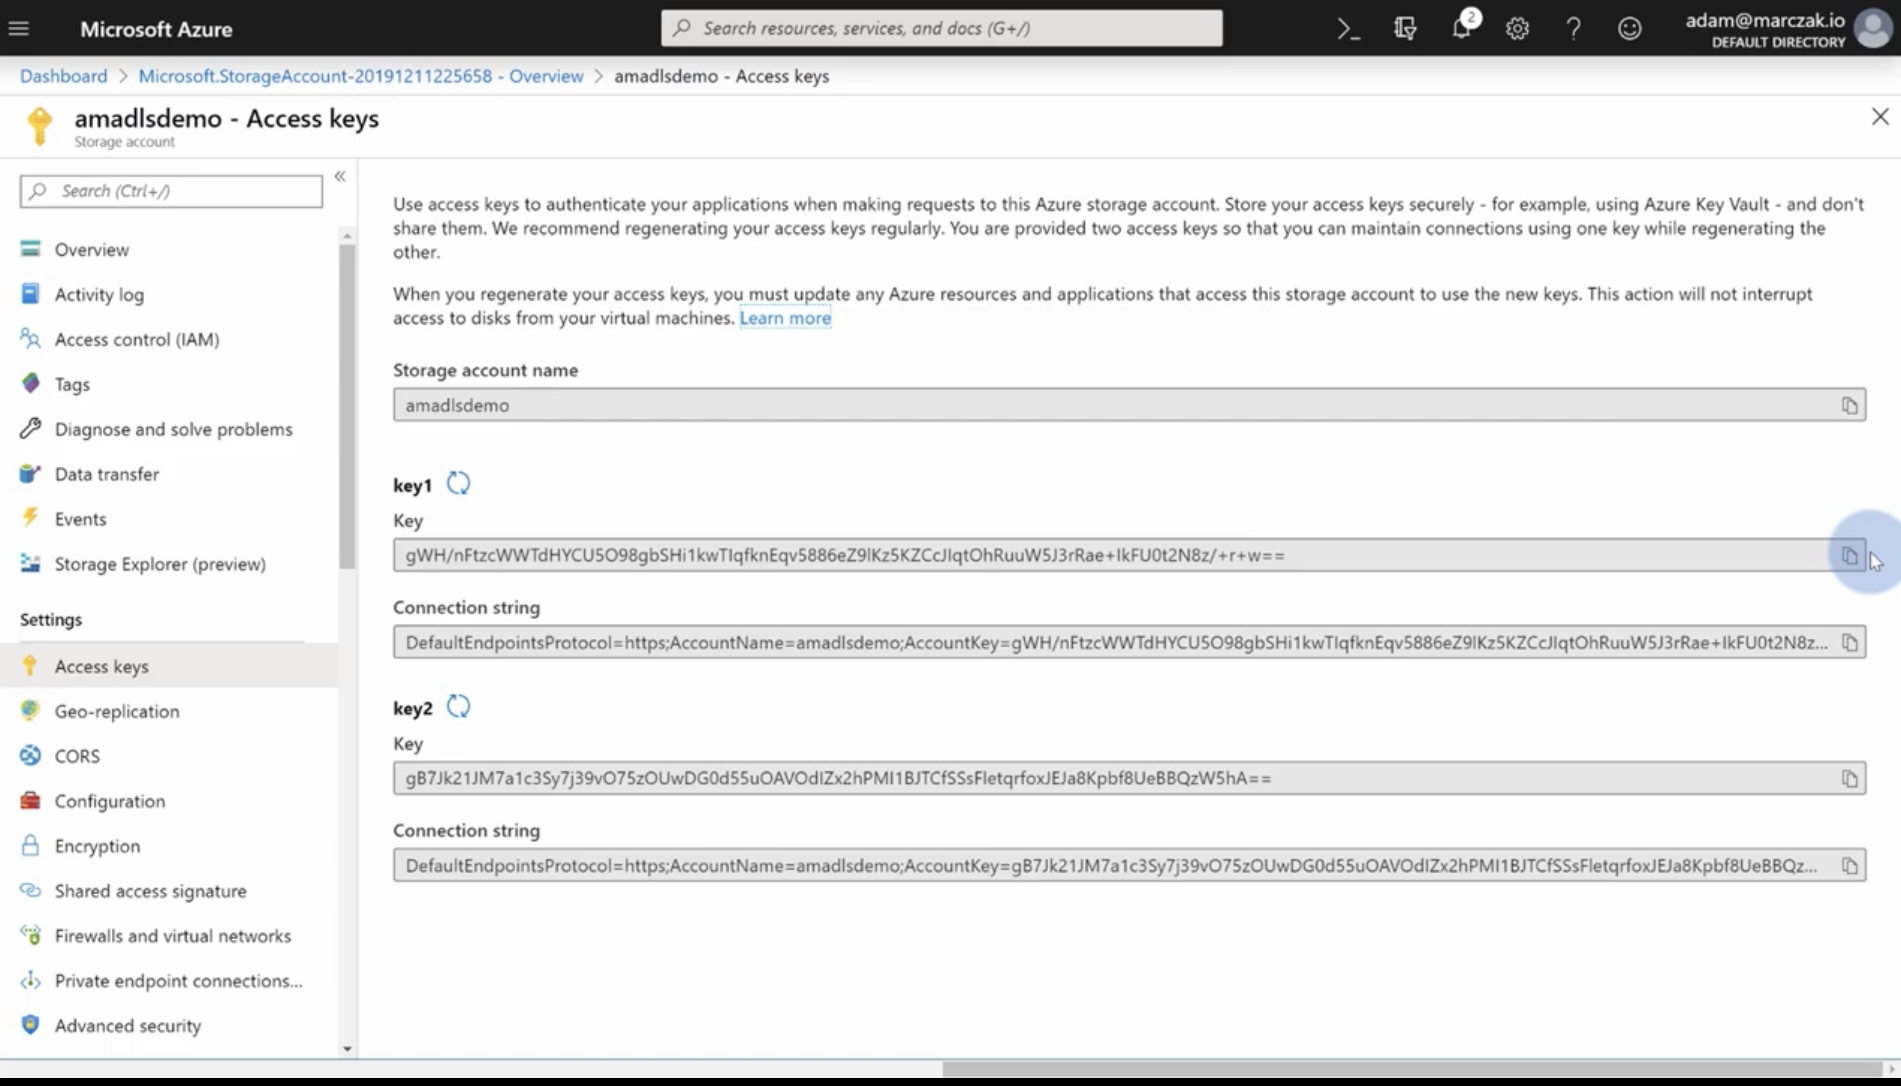
\includegraphics[scale = 0.2]{attachment/chapter_2/Scc127}
\end{figure}

Ebenso kann auch sich mit den Blob Storage verbunden werden.

\begin{figure}[H]
	\centering
	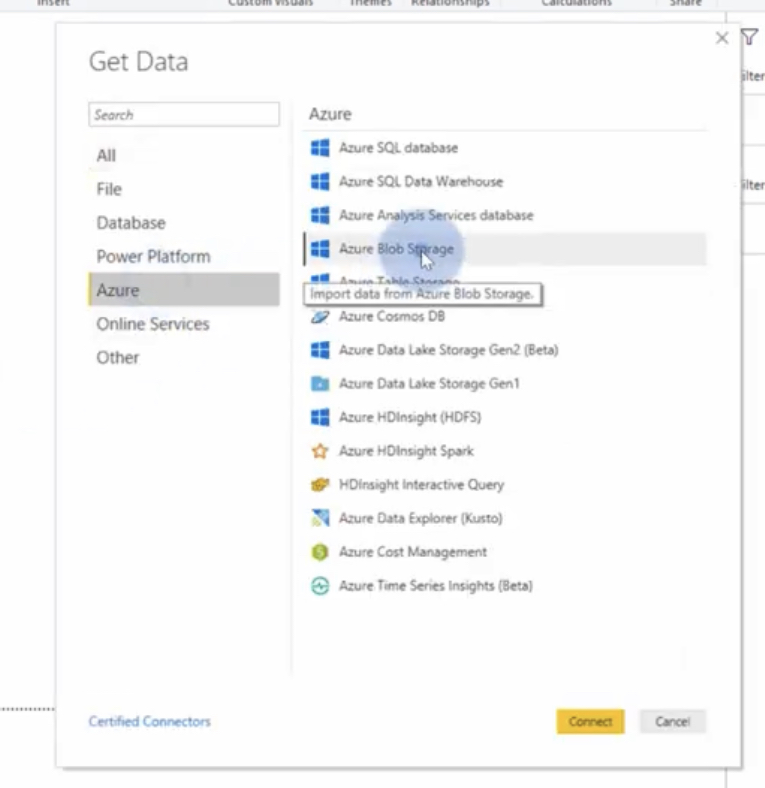
\includegraphics[scale = 0.2]{attachment/chapter_2/Scc129}
\end{figure}

Anstatt die URL anzugeben, kann hier der \textit{Name} des Storage Accounts angegeben werden.

\begin{figure}[H]
	\centering
	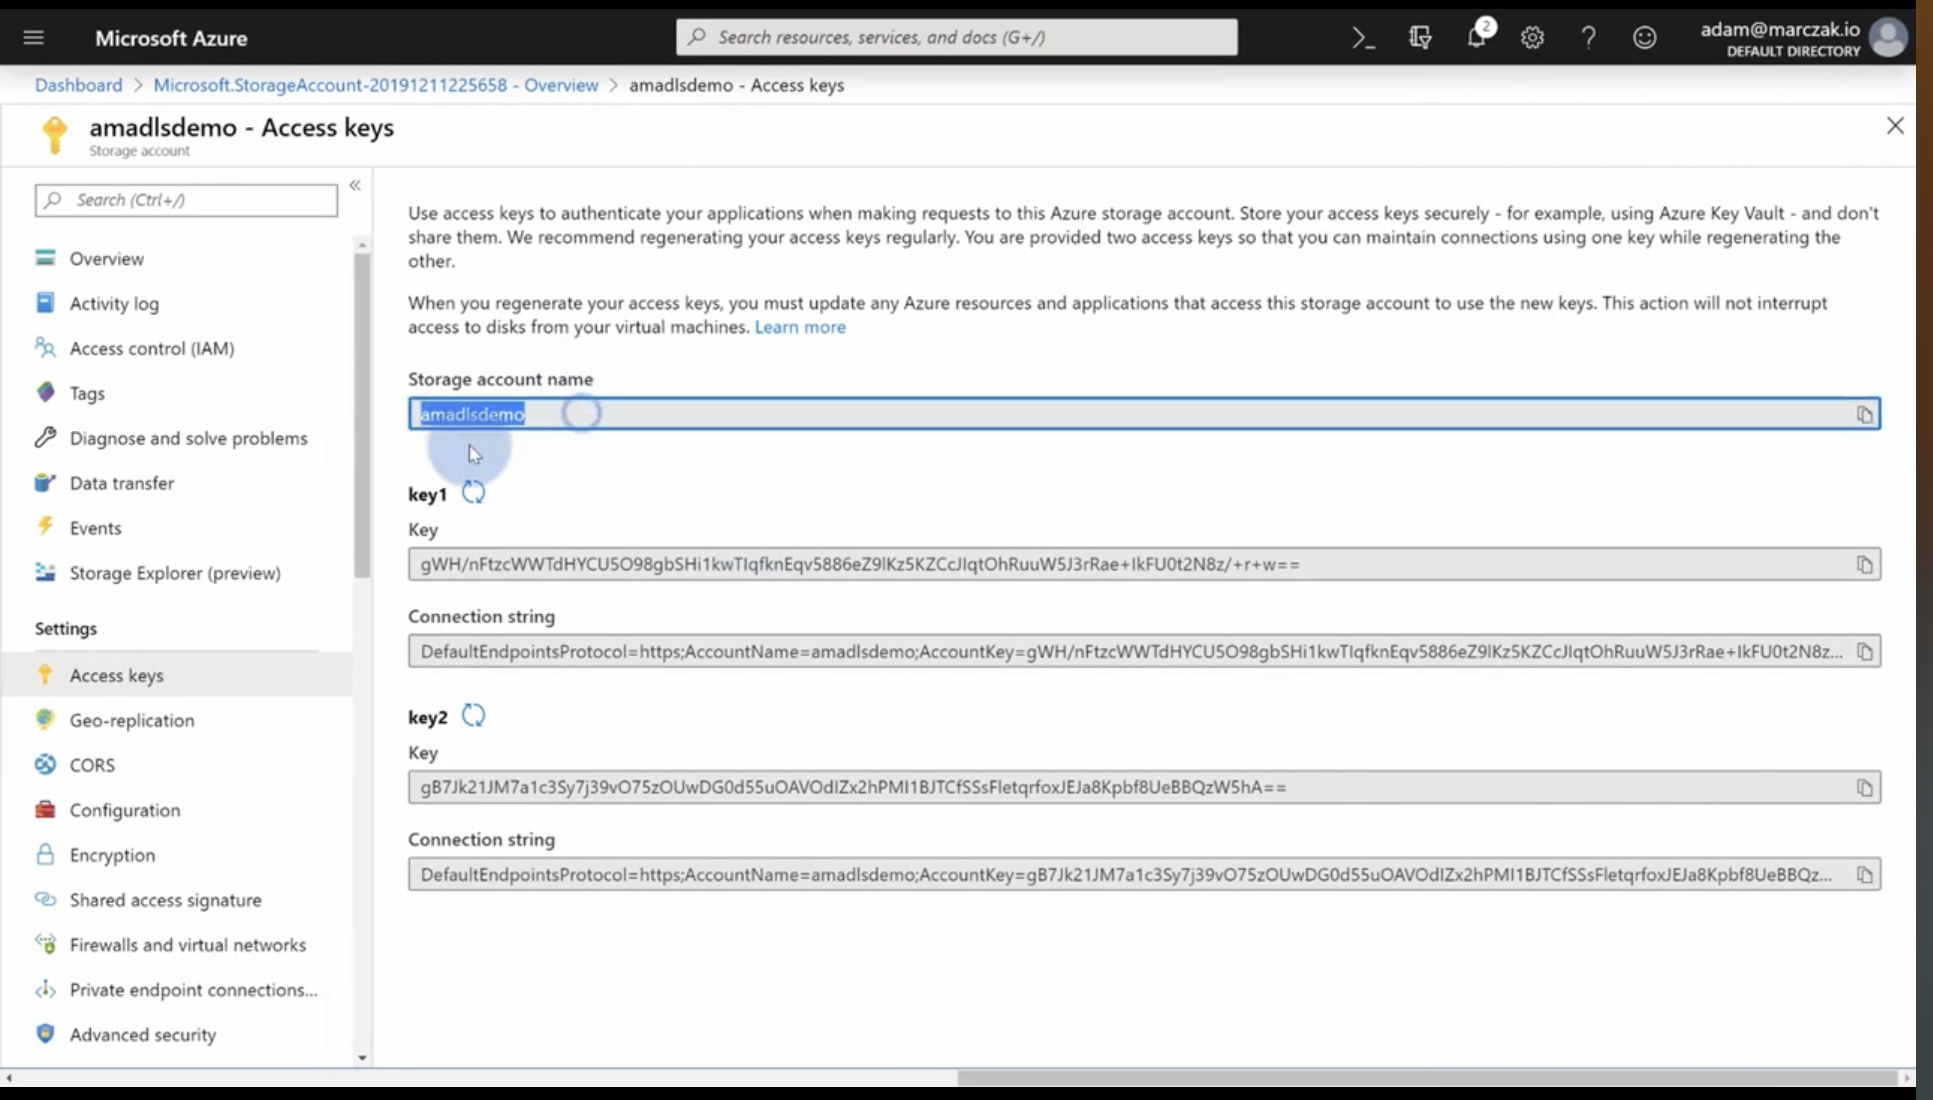
\includegraphics[scale = 0.2]{attachment/chapter_2/Scc130}
\end{figure}

Der gleiche Konto Schlüssel wird hier benötigt. Eine Anmeldung über das Organisationskonto ist nicht für diesen Connector implementiert worden.

\subsection{Big Data Referenz Architektur}
Die drei \textit{V}s von Big Data

\begin{itemize}
	\item Volume - Das Volumen der Daten ist so groß, dass es nicht mehr traditionellen (z.B.: \gls{RDBMS}) Technologien bewältigt werden kann. Z.B.: Sammlung umfangreicher historischen Daten für ein \gls{KI} Modell	
	\item Velocity - Große Datenmengen müssen in Echtzeit oder Quasi-Echtzeit verarbeitet werden.
	\item Variety - Daten können in traditioniellen und nicht traditioniellen Formen vorliegen.
\end{itemize}

\section{Azure Data Lake Storage Gen 2}

Dieses Produkt ist ein \gls{PaaS}. Es bietet größtmöglichen Speicher. Es werden Billionen von Dateien, welche mit der parallel Rechenleistung Gigabyte an Durchlauf ermöglicht. Es handelt sich hier um eine Erweiterung von \textit{Azure Blob Storage}.\\

Für \gls{ADL} wird je nach Kontext Verkürzungen verwendet, siehe die Beispiele Data Lake, Azure Lake, Azure Data Lake, Azure Gen 2.


\subsection{Unterschiede zu Blob Storage}\label{subsec_Unterschied_Blob_Storage}
\begin{itemize}
	\item Struktur
			\begin{itemize}
				\item \textit{Azure Gen 2:} Hierarchische Namensstruktrur (Wie ein Ordner System)
				\item \textit{Blob Storage:} Flat namespace object store
			\end{itemize}
	\item Zweck (Purpose)
			\begin{itemize}
				\item \textit{Azure Gen 2:} Optimiert Speicherung für Big Data Analyse
				\item \textit{Blob Storage:} Allgemeine Scenarios für Big Data Speicherung, inkl. Daten Analyse
			\end{itemize}
	\item Performance (Analysis)
			\begin{itemize}
				\item \textit{Azure Gen 2:} Bessere Daten Ladung (Retrieval)
				\item \textit{Blob Storage:} Gute Daten Ladung (Retrieval)
			\end{itemize}
	\item Kosten (Cost)
			\begin{itemize}
				\item \textit{Azure Gen 2:} Geringe Kosten für Analyse
				\item \textit{Blob Storage:} Höhere Kosten für Analyse
			\end{itemize}
\end{itemize}\footnote{
	\href{https://medium.com/awesome-azure/azure-difference-between-azure-blob-storage-and-azure-data-lake-storage-comparison-azure-blob-vs-adls-gen2-81af5ef2a6e1}{Quelle}
}

\subsection{Setting Up}
Der Azure Data Lake weißt sich über ein Symbole mit einer gewellten Linie (Symbolisieren von Wasser) aus.

\begin{figure}[H]
	\centering
	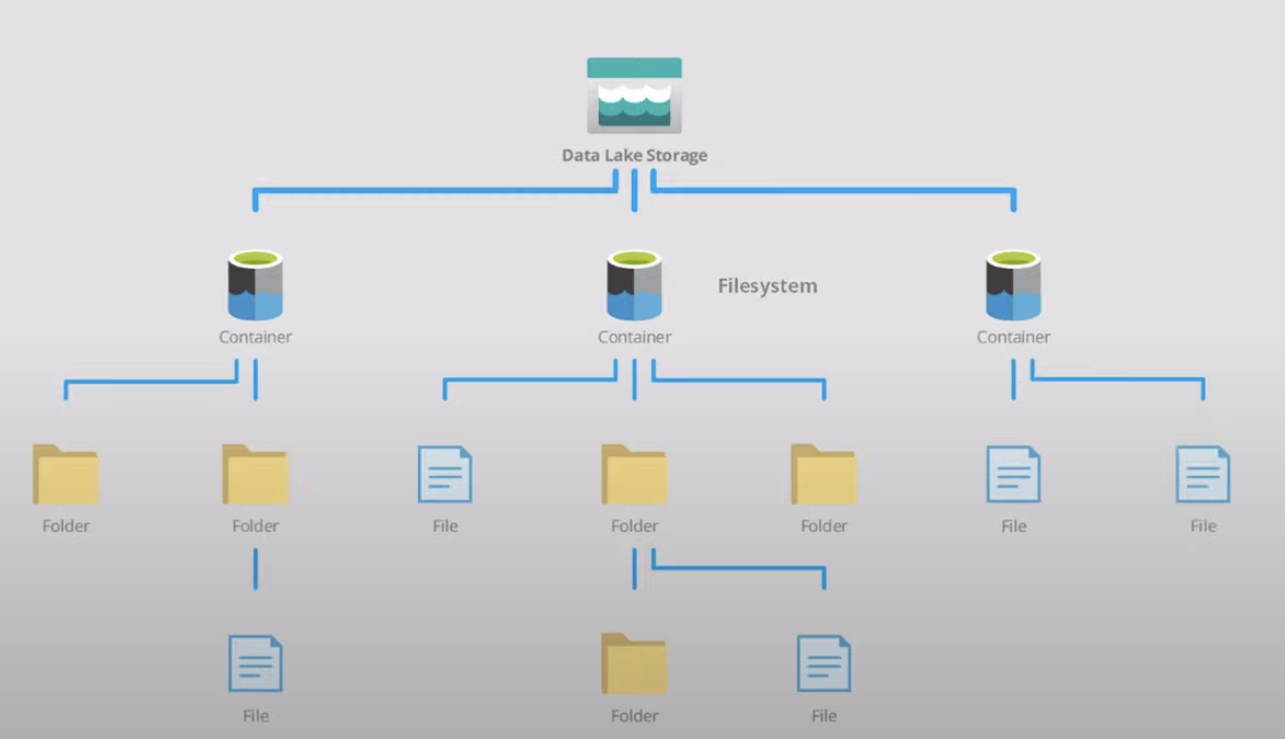
\includegraphics[scale = 0.5]{attachment/chapter_2/Scc110}
\end{figure}

In dem Lake können verschiedenen Container (File System) angelegt werden. - Diese haben ebenso, eine gewellte Linie im Zentrum. In jedem Container können Dateien und Ordner angelegt werden. Anders als in einem regulären \gls{g_DataLake} ermöglicht Azure eine Hierachie in den Daten mit Ordner zu ermöglich.\\

Um einen \gls{ADL} einzurichten, wird dieser genauso wie ein \textit{Azure Blob Storage} erstellt:

\begin{figure}[H]
	\centering
	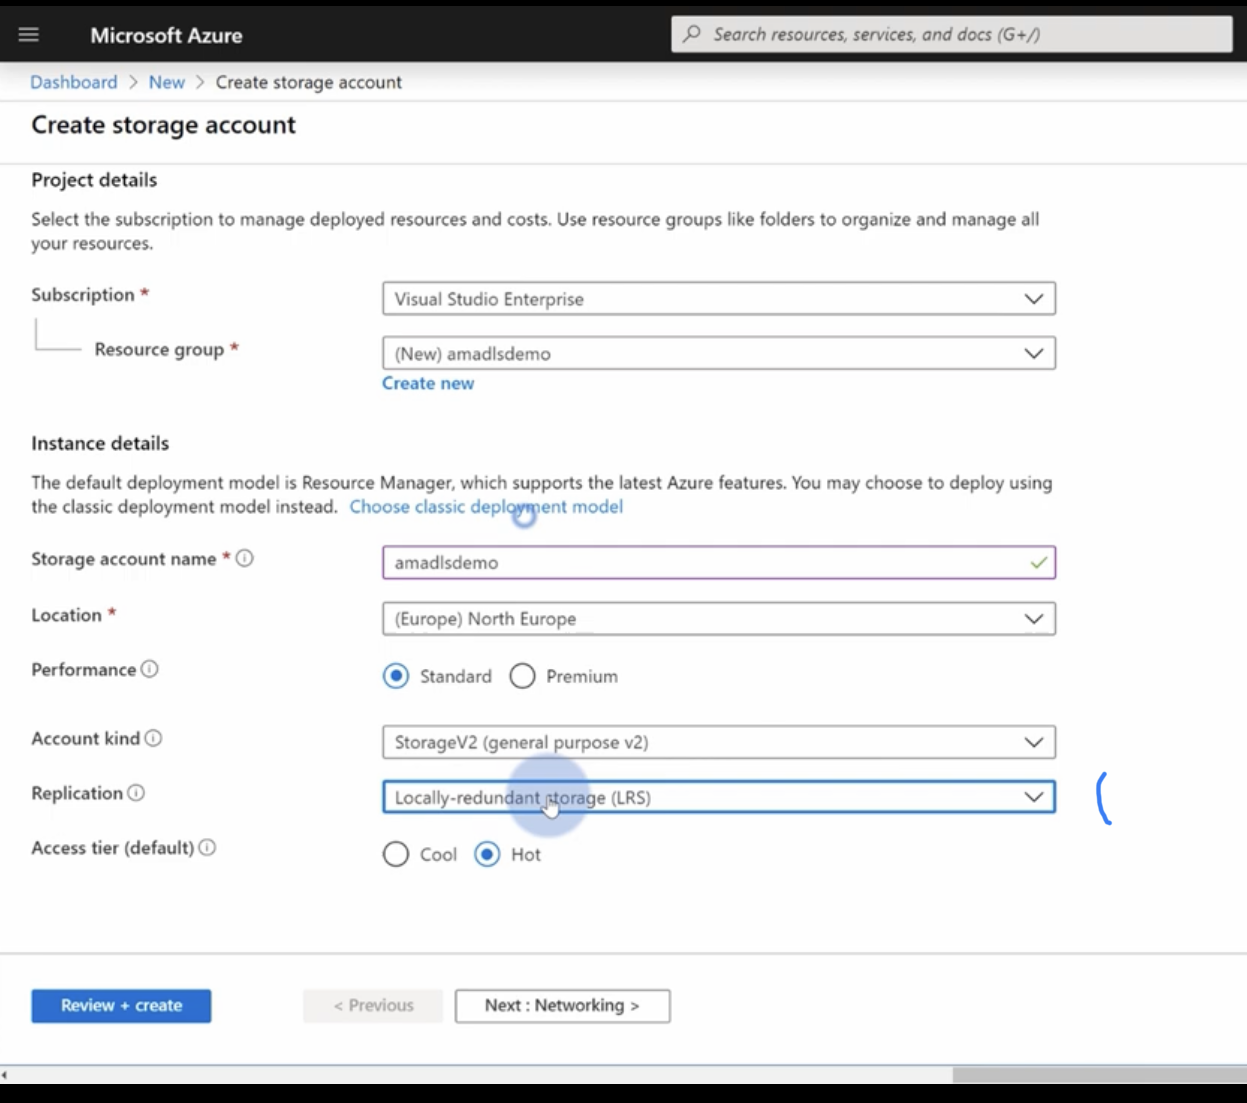
\includegraphics[scale = 0.4]{attachment/chapter_2/Scc112}
\end{figure}

\begin{itemize}
	\item Mit der Einstellung \textit{Access Tier} kann zwischen \textit{Hot} oder \textit{Cold} unterschieden werden. Dies regelt die Zugriffsgeschwindigkeit. Je schneller der Zugriff ermöglicht wird, desto teuer die Verbrauchskosten.
	\item Mit \textit{Replication} kann ebenso der Storage Account auf auf Schnelligkeit eingestellt werden.
	\item Der Account Type unterscheidet zwischen Premium und General Purpose V2 Accounts.
	\begin{figure}[H]
	\centering
	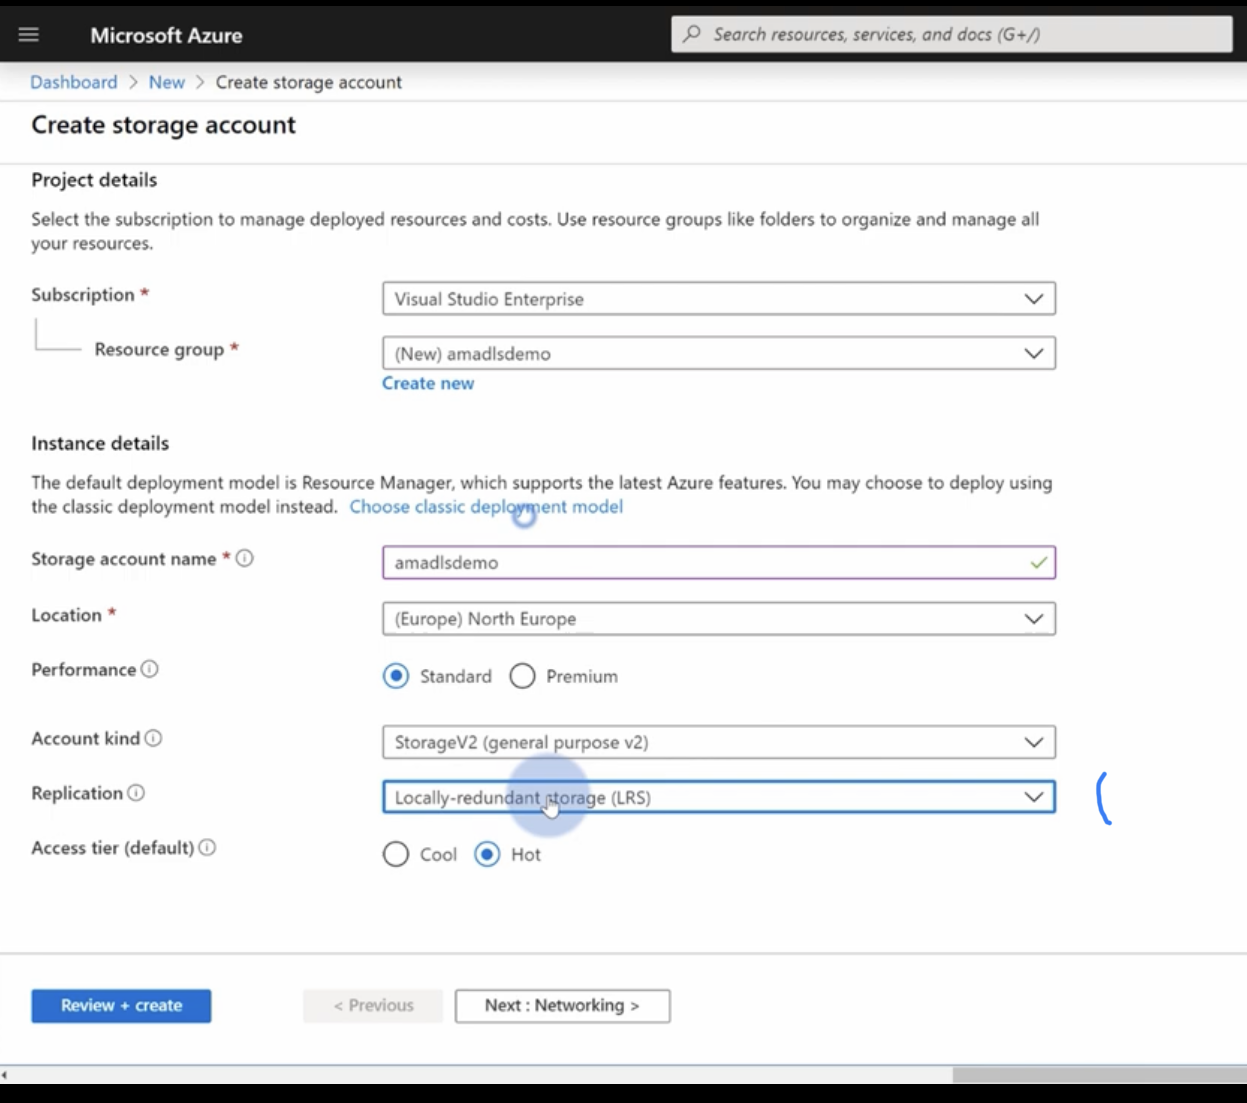
\includegraphics[scale = 0.4]{attachment/chapter_2/Scc112}
\end{figure}
	\item Um die einen \gls{ADL} zu ermöglichen, muss unter \textit{Advance} die Option \textit{Hierachiacal Namespace} ausgewählt werden. 
	\href{https://learn.microsoft.com/en-us/azure/storage/common/storage-account-create?toc=%2Fazure%2Fstorage%2Fblobs%2Ftoc.json&tabs=azure-portal}{Quelle}

\begin{figure}[H]
	\centering
	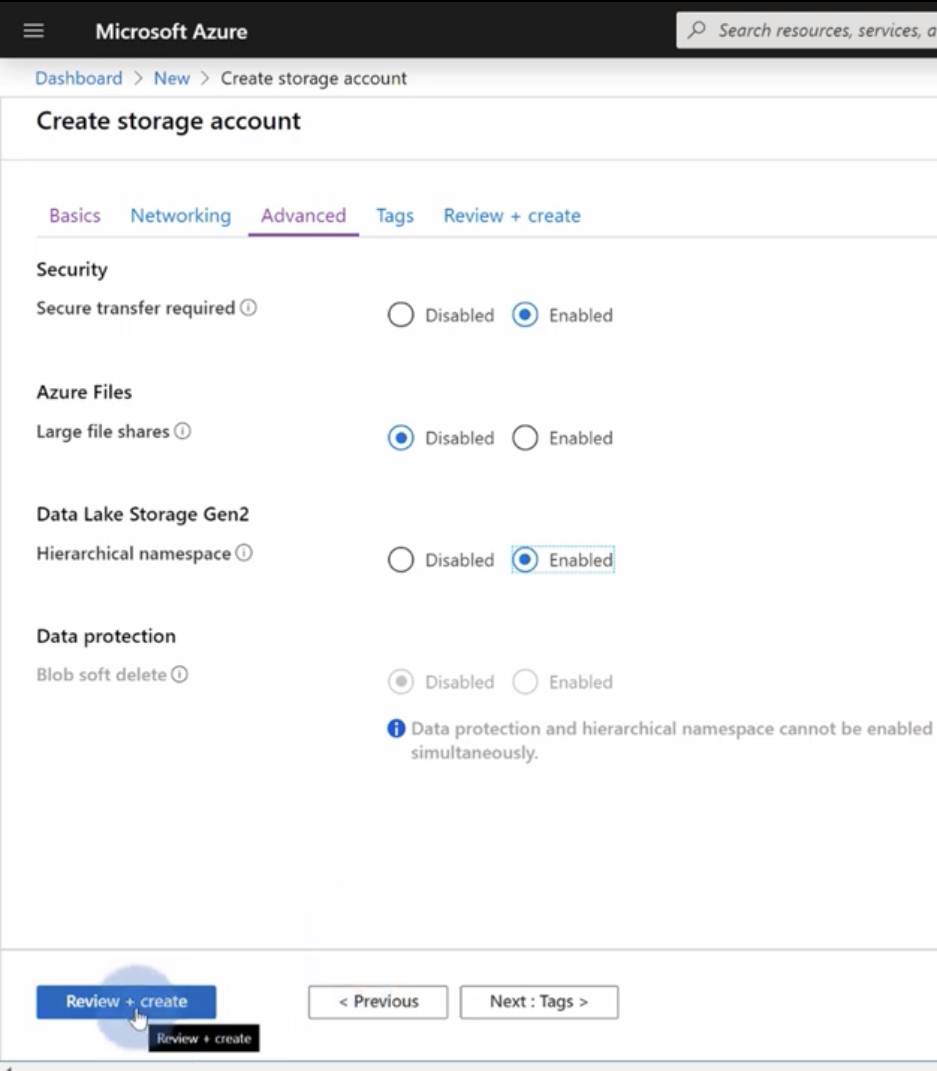
\includegraphics[scale = 0.2]{attachment/chapter_2/Scc113}
\end{figure}
\end{itemize}


Ist der \gls{ADL} eingerichtet, ist der Unterschied zu einem regulären Blob Storage über das Icon für den Container erkennbar.

\begin{figure}[H]
	\centering
	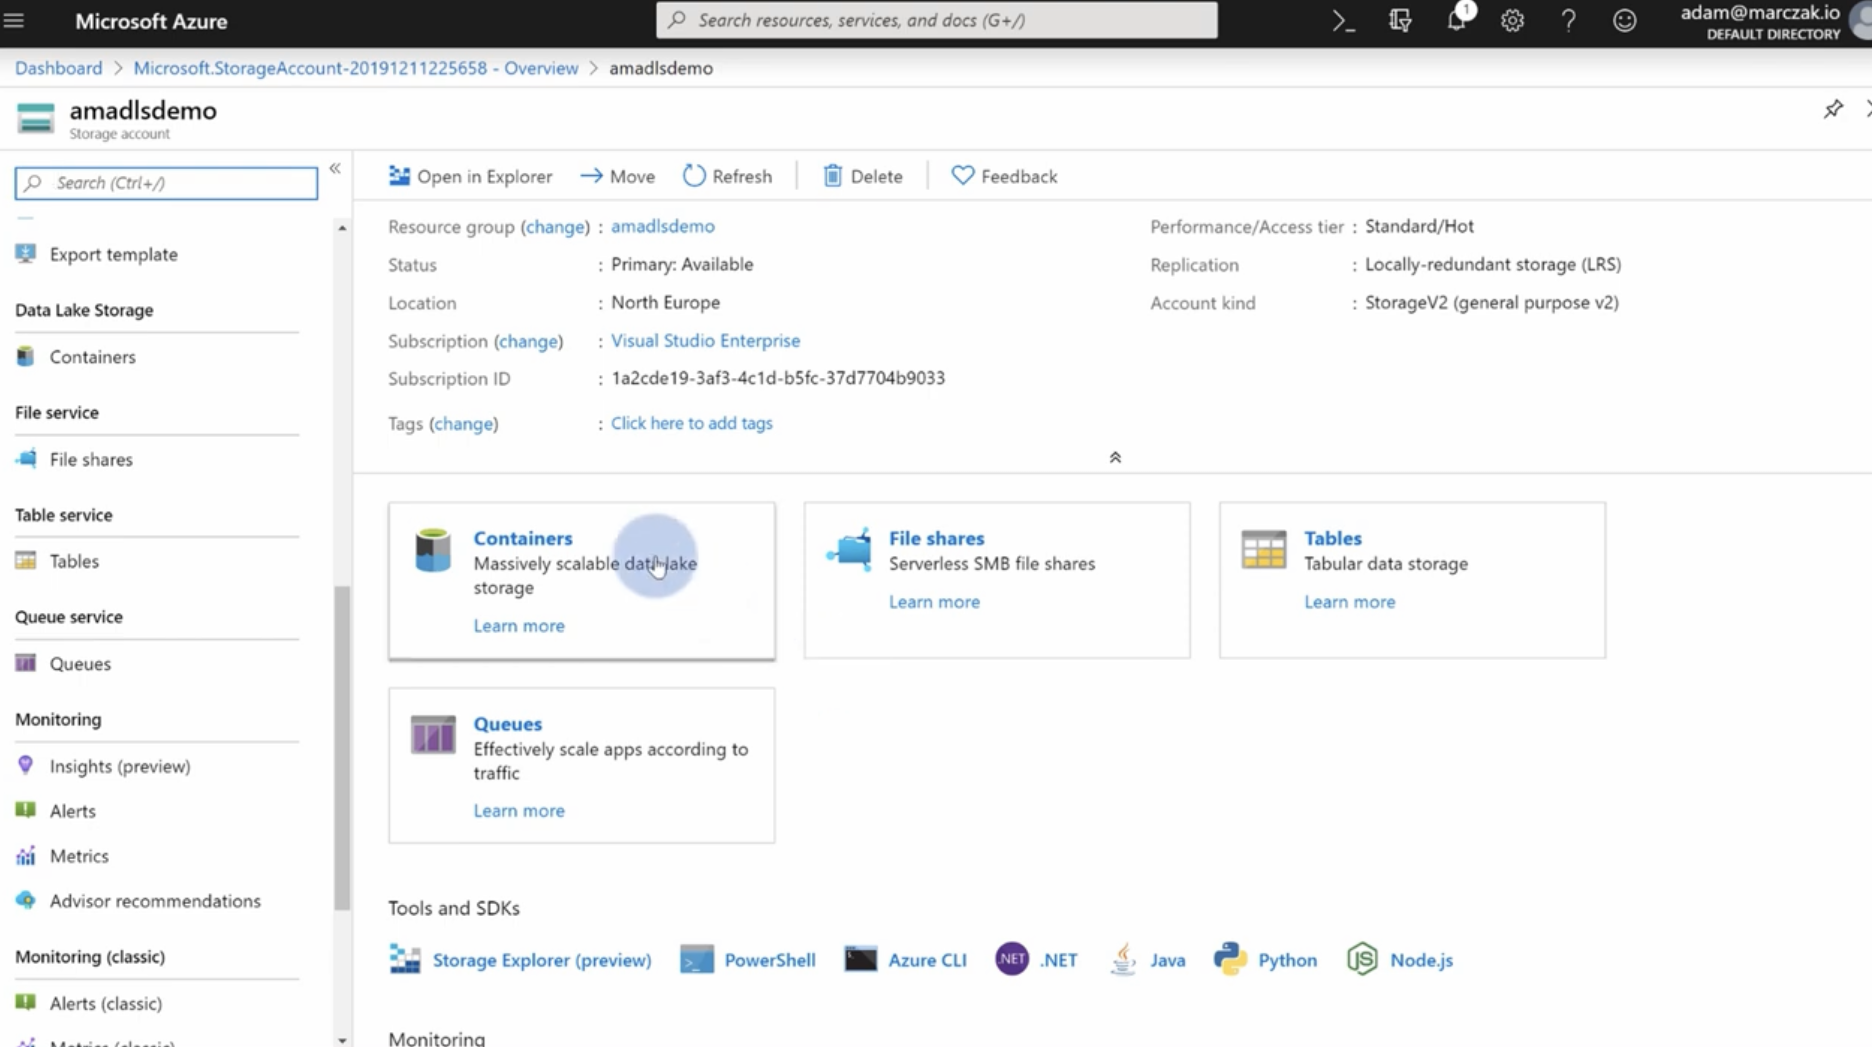
\includegraphics[scale = 0.3]{attachment/chapter_2/Scc114}
\end{figure}

Über der Überkategorie \textit{Container} können neuen File Systems (Container) eingerichtet werden.

\begin{figure}[H]
	\centering
	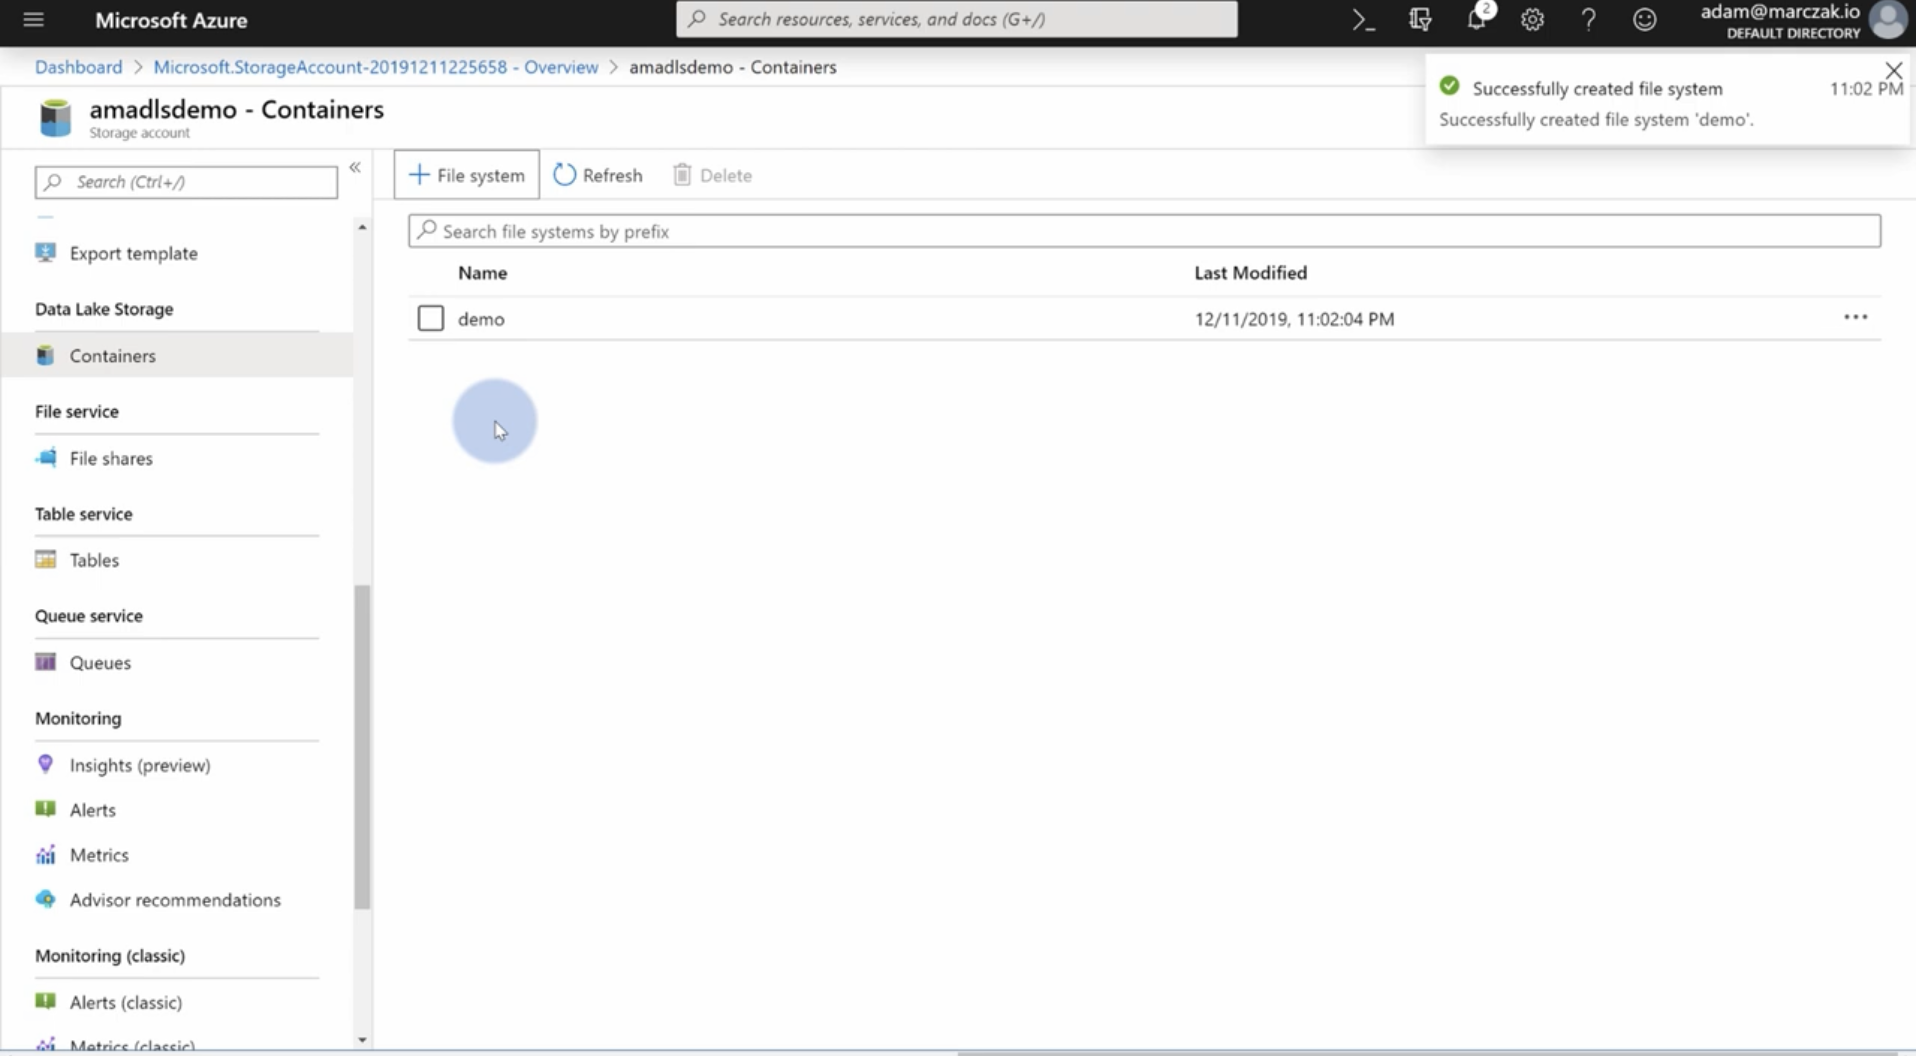
\includegraphics[scale = 0.3]{attachment/chapter_2/Scc115}
\end{figure}




\section{Azure Key Vault}
\subsection{Allgemein}
Azure Key Vault ermöglicht \textit{Keys, Secrets und Zertifikate} zu speichern.

\begin{figure}[H]
	\centering
	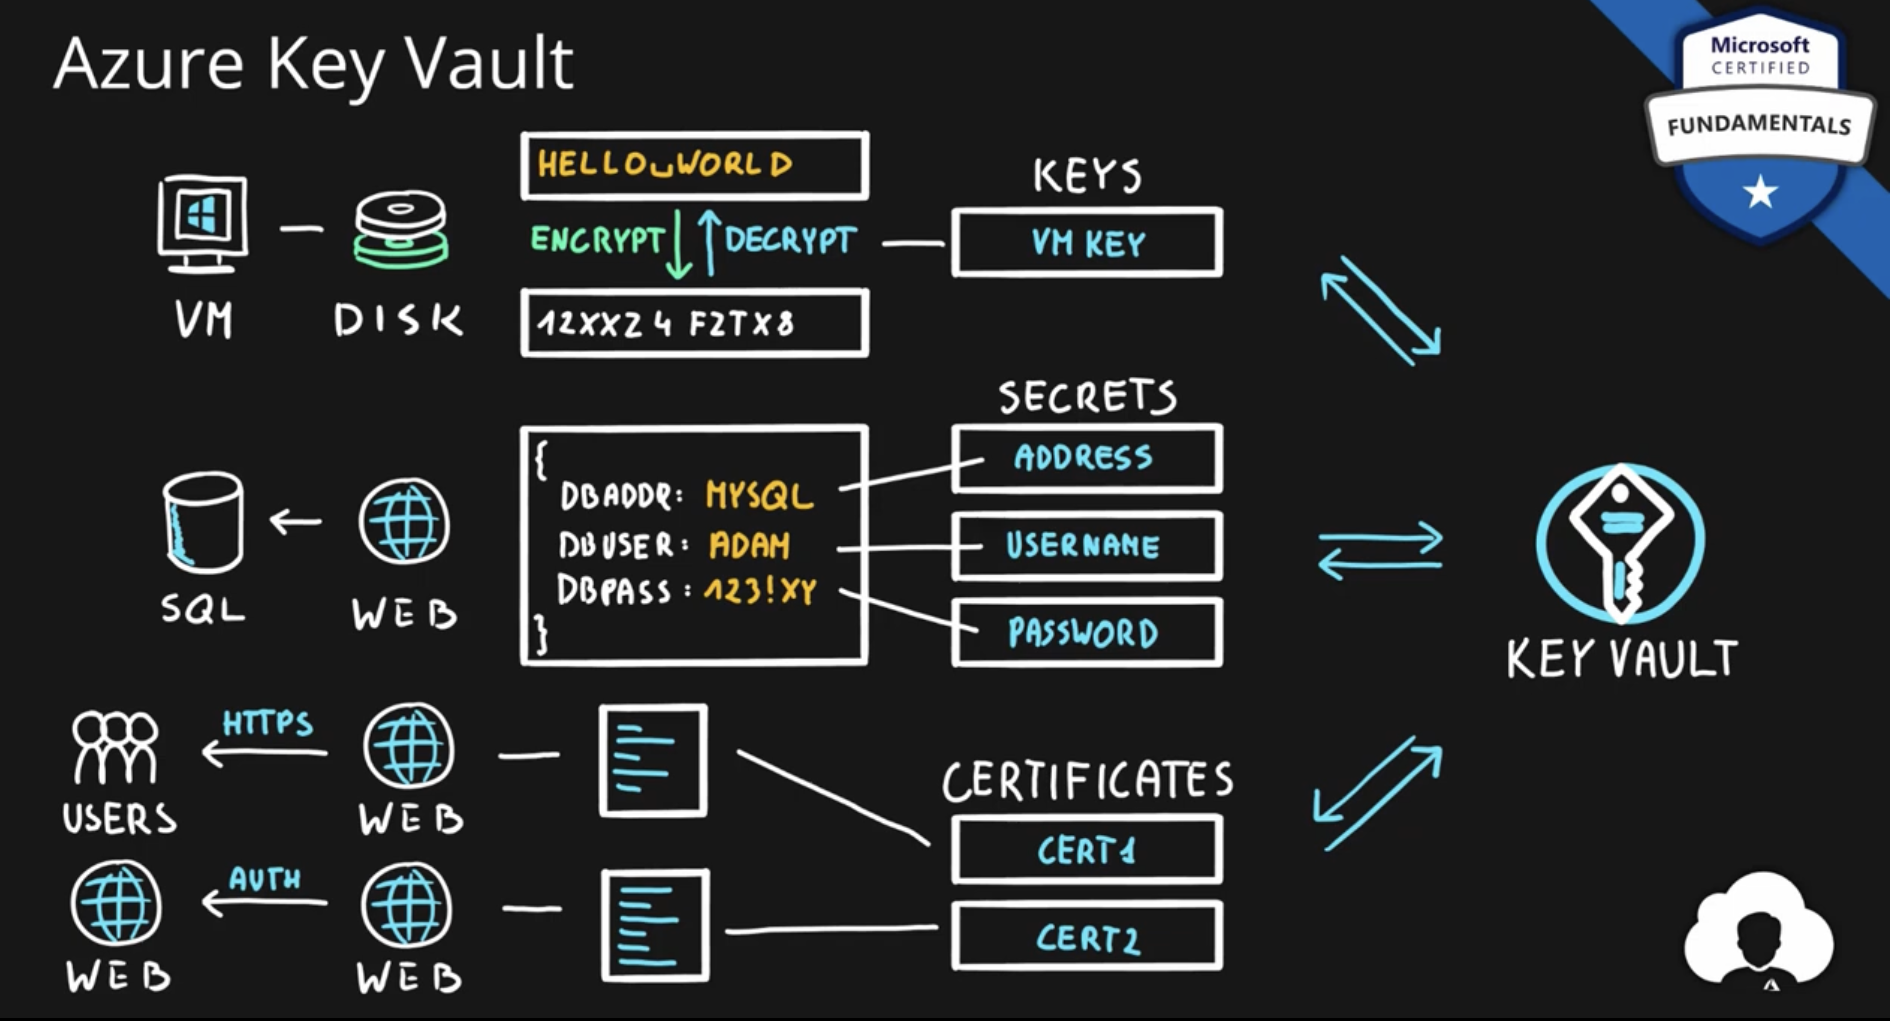
\includegraphics[scale = 0.2]{attachment/chapter_2/Scc131}
	\caption{Azure Key Vault Funktionalitäten}
\end{figure}

Als Beispiele können Keys Verschlüsselung von Information ermöglichen, Secrets Zugriff auf andere Systeme ermöglichen und Zertifikate Authentifizierung von Usern ermöglichen.\\

Im Azure Portal ist unter der Ressource vier Einstellungen einsehbar
\begin{itemize}
	\item Keys,
	\item Secrets,
	\item Certificate,
	\item Access Policies
\end{itemize}

Die ersten drei haben keine erweiterte Struktur. In einer flachen Liste können je Kategorie Einträge geschrieben werden.
\begin{figure}[H]
	\centering
	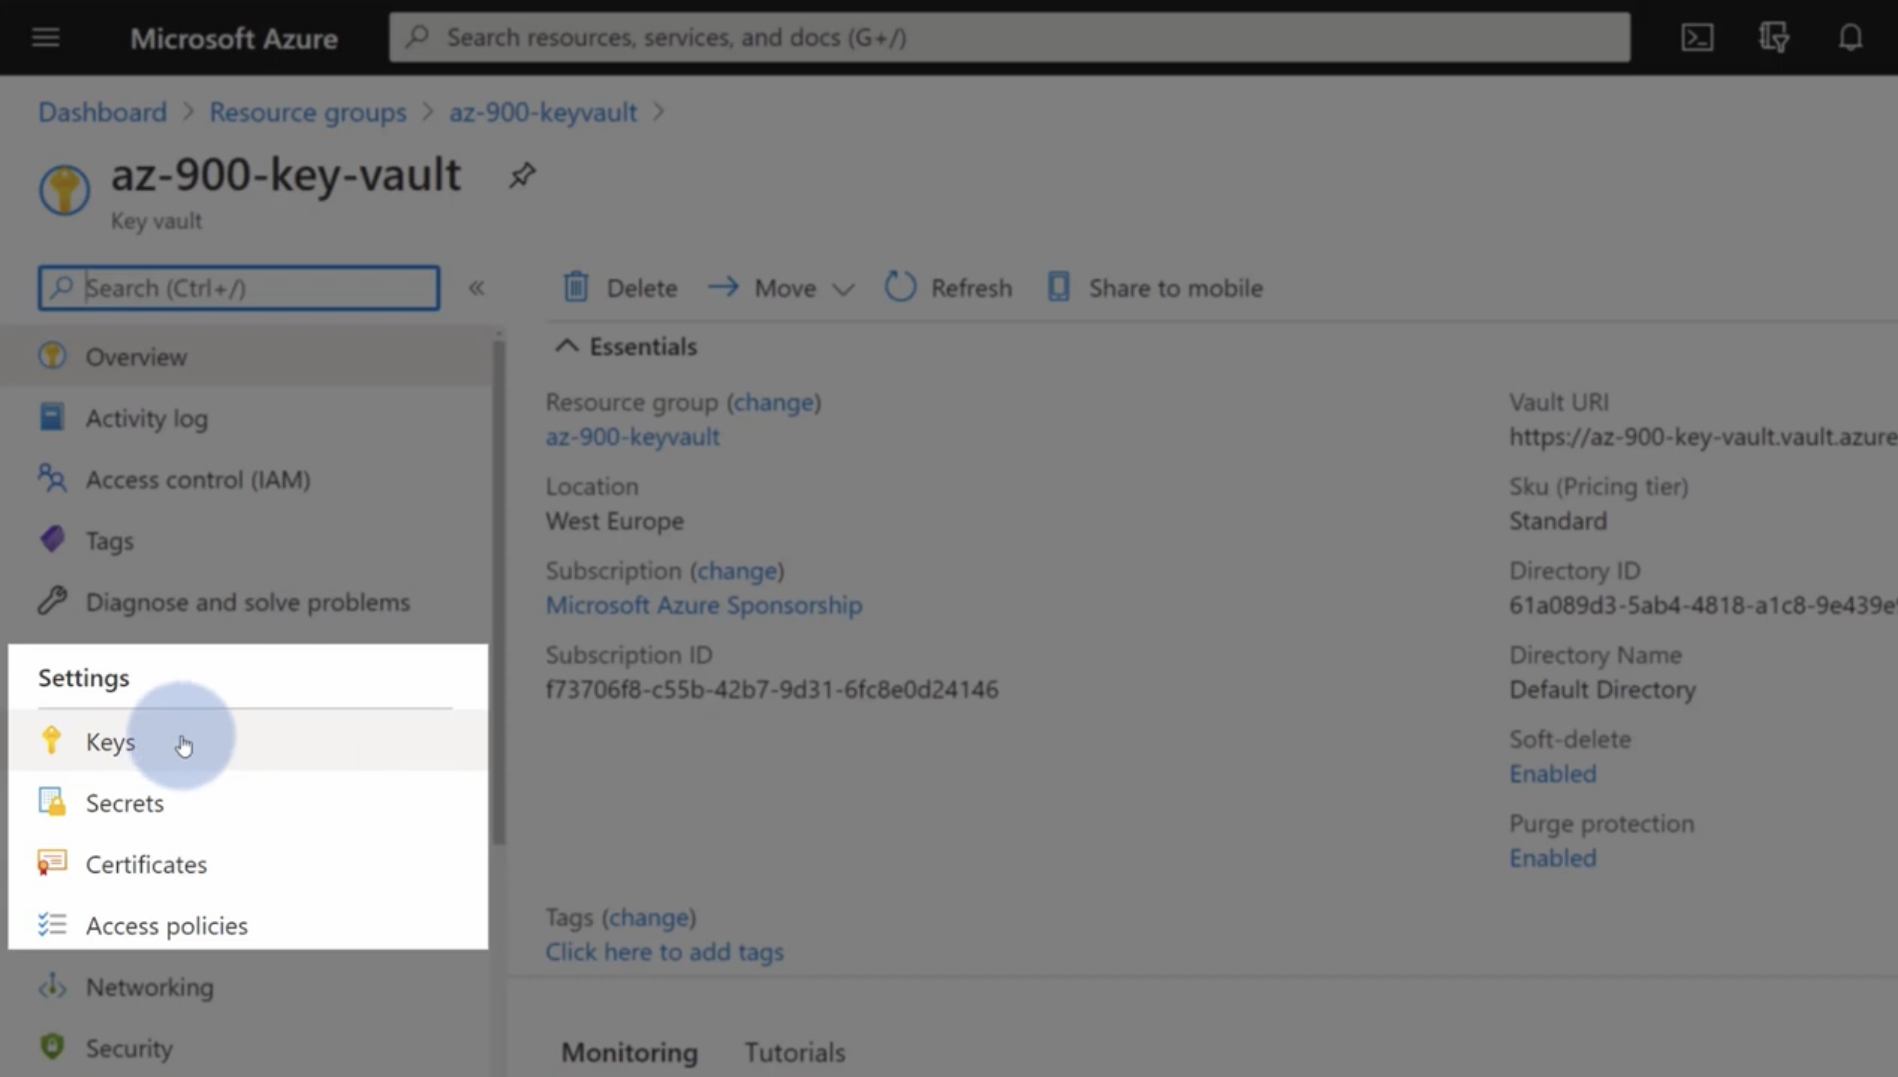
\includegraphics[scale = 0.2]{attachment/chapter_2/Scc132}
	\caption{Azure Portal Ressourcen Einsicht für Azure Key Vault}
\end{figure}

Bei der Anlegung eines Key/Secrets/Certificate können neben dem eigentlichen Werte auch Fristen und der allgemeine Zugriff eingestellt werden.
\begin{figure}[H]
	\centering
	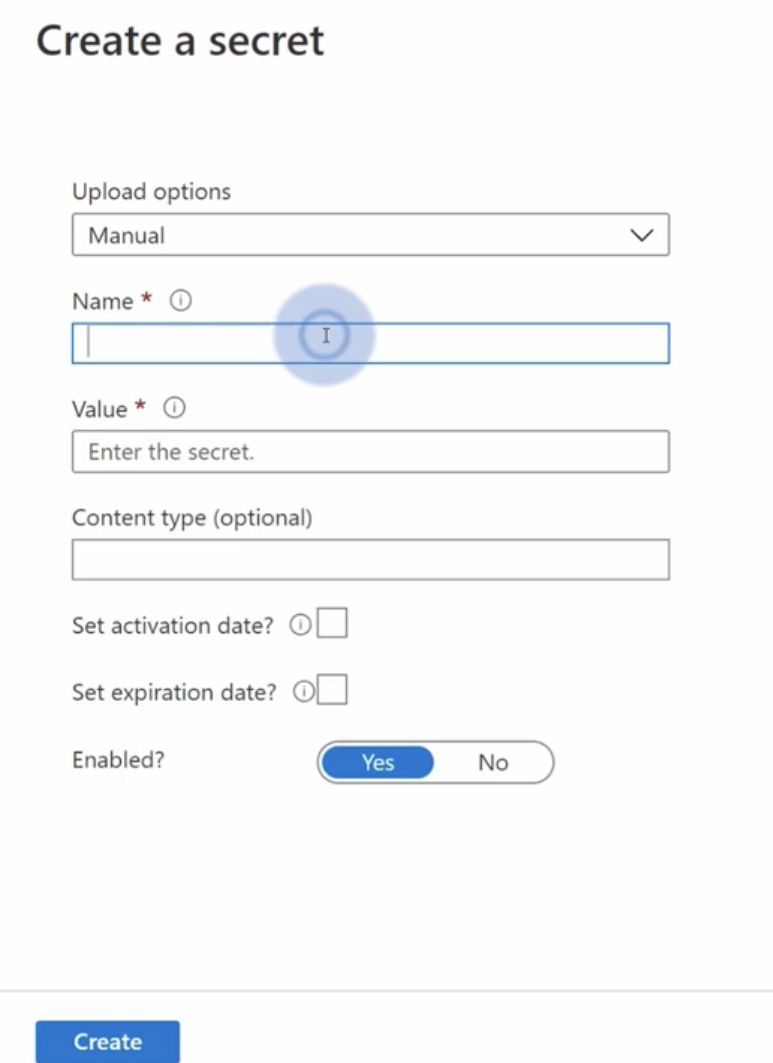
\includegraphics[scale = 0.2]{attachment/chapter_2/Scc133}
	\caption{Anlegen eines Secrets}
\end{figure}

\subsection{Versionierung}
Für jeden Eintrag ist ein Versionsverlauf bereitgestellt. Am Beispiel von dem Secret Eintrag \textit{mysecret} ist beim Anklicken eine Versiosnummer einsehbar. In der ersten Spalte wird die aktuelle Versionsnummer angezeigt.

\begin{figure}[H]
	\centering
	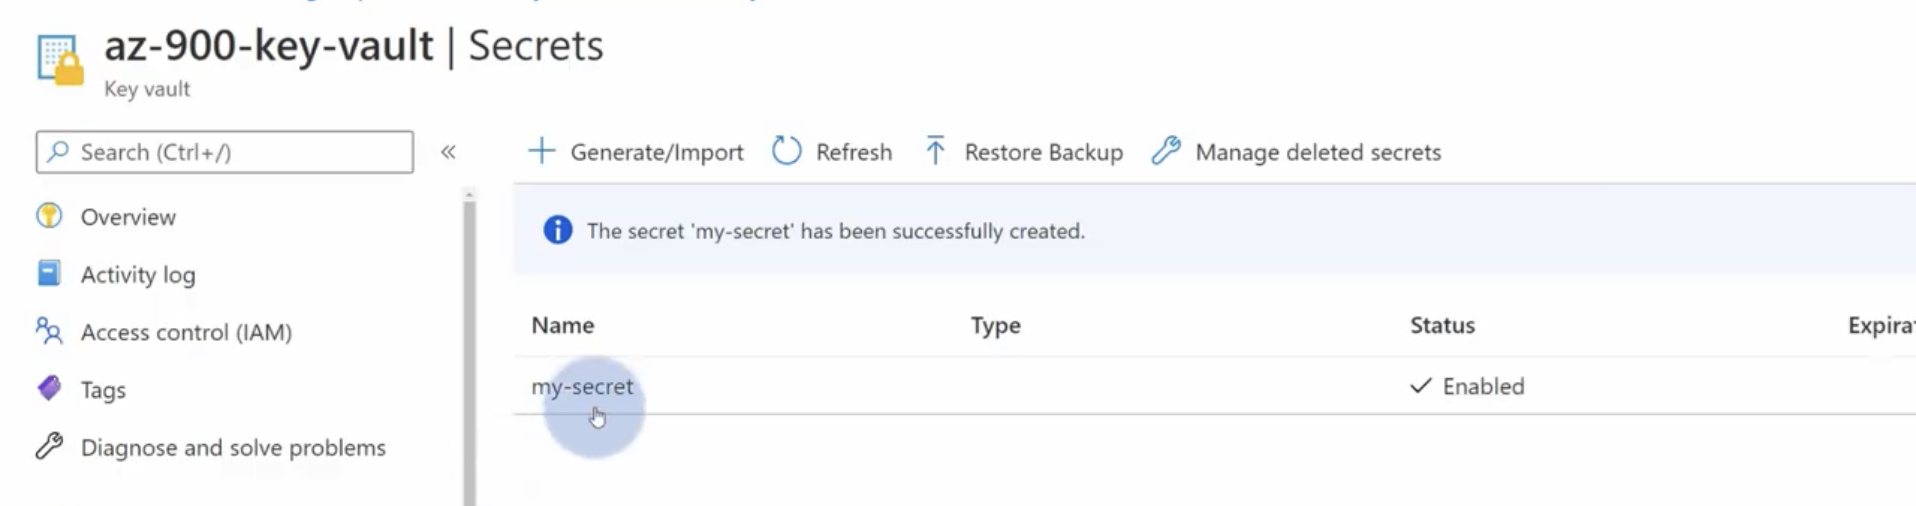
\includegraphics[scale = 0.2]{attachment/chapter_2/Scc134}
	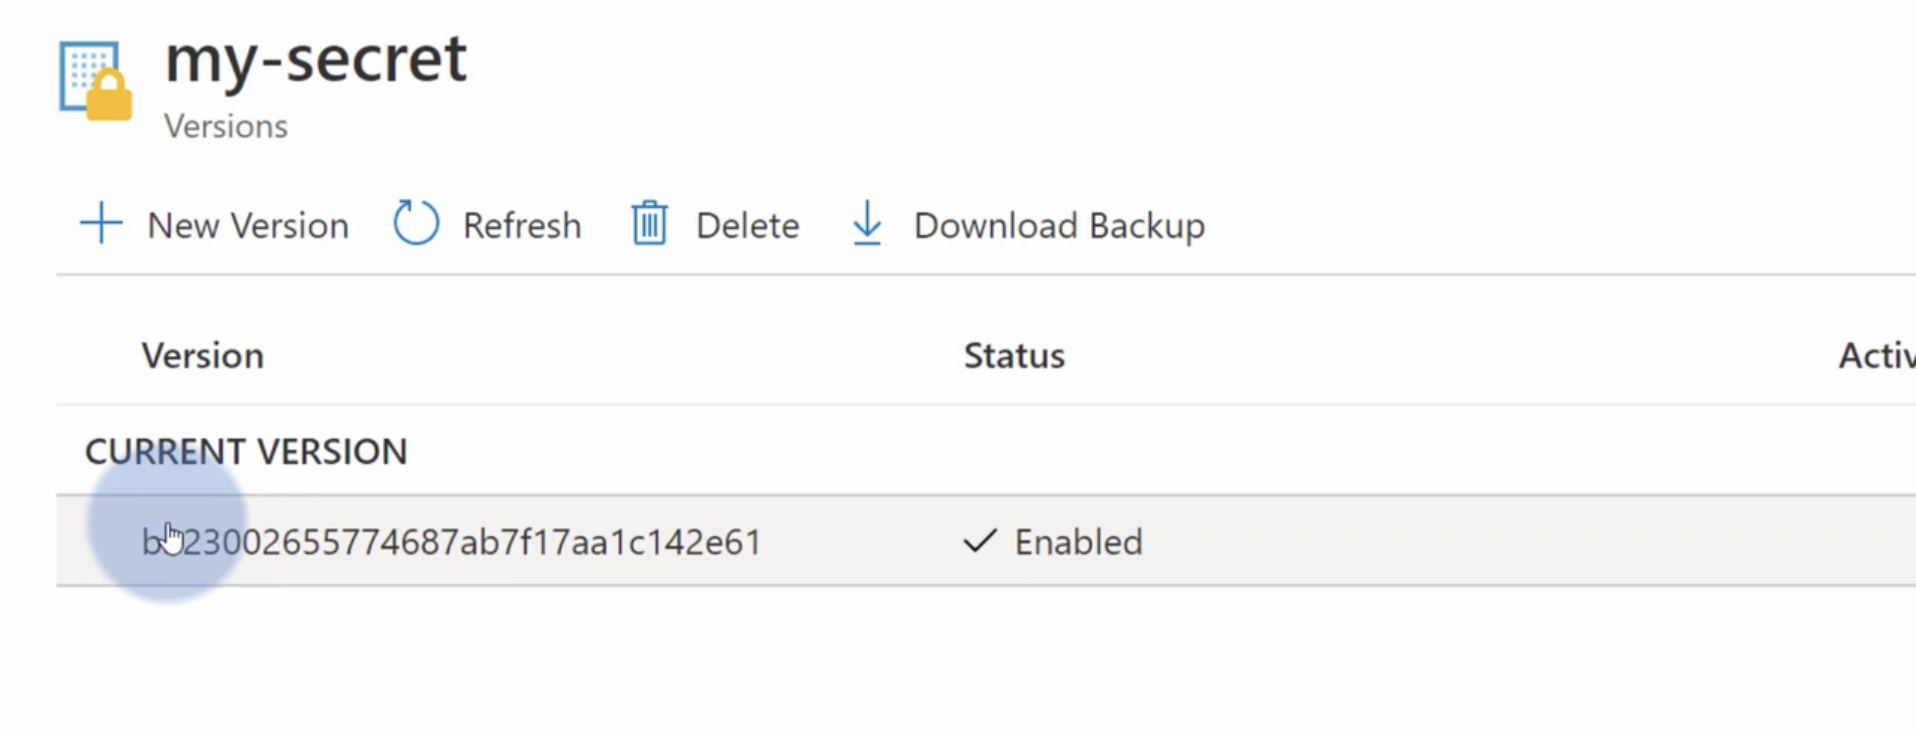
\includegraphics[scale = 0.2]{attachment/chapter_2/Scc135}
	\caption{\textit{mysecret} in der Liste mit Details}
\end{figure}

Wird auf die aktuelle Version geklickt, ist der Secrete Identifiy einsehbar. Dieser ist eine URL, welcher auf das Secret zu der aktuellen Version zeigt.

\begin{figure}[H]
	\centering
	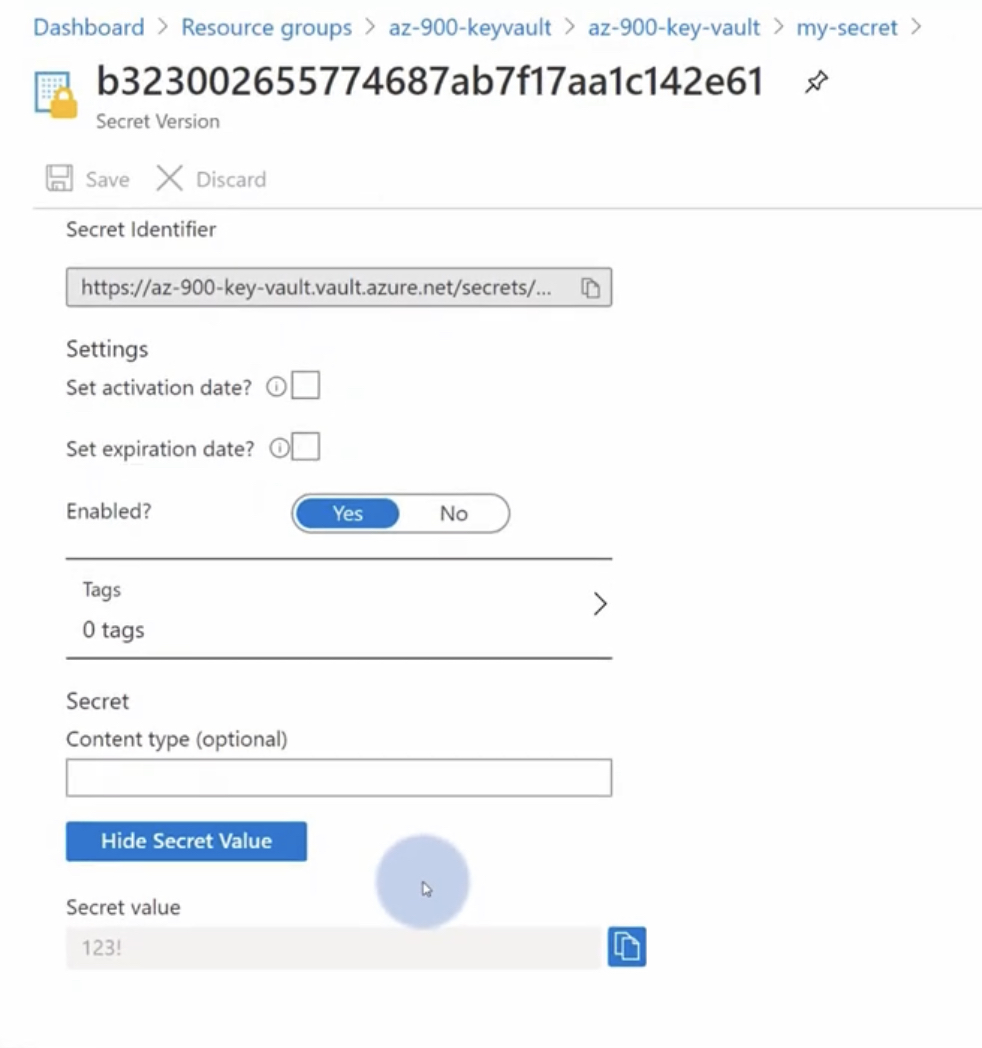
\includegraphics[scale = 0.2]{attachment/chapter_2/Scc136}
	\caption{Versionierung eines Secrets}
\end{figure}
